\documentclass[11pt, a4paper]{article}
\PassOptionsToPackage{fleqn}{amsmath}

\usepackage[T1]{fontenc}
\usepackage[english]{babel}

% --- Fonts --------------------------------------------------------------------
% Serif (main text)
\usepackage{erewhon}

% Sans (headings, small UI, captions). sfdefault -> \sffamily becomes default sans.
\usepackage[sfdefault]{FiraSans}

% Monospace (code/listings)
\usepackage{FiraMono}

% Math font: newtxmath is a dependable pdfLaTeX math package.
% Some useful options you can try: upint, varg, slantedGreek, smbb, cmintegrals.
% Example: \usepackage[upint,slantedGreek]{newtxmath}
\usepackage[upint]{newtxmath}

% Micro-typography (always recommended for professional docs)
\usepackage{microtype}
\microtypesetup{protrusion=true,expansion=true}

% Math, Physics
\usepackage{mathtools}
\usepackage{amsfonts}
\usepackage{physics, tensor}

% Margins and spacing
\usepackage{geometry}
\geometry{left=25mm, right=25mm, top=30mm, bottom=30mm, headheight=15pt}
\usepackage{setspace}
\singlespacing % or \onehalfspacing or \doublespacing

% Misc
\usepackage{xcolor}
\usepackage[none]{hyphenat}
\usepackage[colorlinks=true,
  linkcolor=black,
  citecolor=blue!60!black,
  urlcolor=blue!60!black
]{hyperref}
\usepackage{cleveref}
\usepackage{ulem}

\usepackage{tikz}
\usetikzlibrary{arrows.meta}

\tikzset{
  qnode/.style={circle, draw, minimum size=18pt, inner sep=1pt},
  qarr/.style={-Latex, thick}
}
\newcommand{\qvertices}{
  \node[qnode] (1) at (90:1.05) {$1$};
  \node[qnode] (2) at (210:1.05) {$2$};
  \node[qnode] (3) at (330:1.05) {$3$};
}

% Titles
\usepackage{titlesec}
\titleformat
{\section} % command
{\sffamily\bfseries\Large} % format
{\thesection.} % label
{1ex} % sep
{} % before-code
[] % after-code

% Title page
\usepackage{titling}
\pretitle{\LARGE\bfseries\sffamily\noindent}
\posttitle{
    \par
    \noindent\makebox[\linewidth]{\rule{\linewidth}{1pt}}
    \vspace{2ex}
}
\preauthor{
    \par\large\bfseries\sffamily\noindent
}
\postauthor{\par}
\predate{\par\vspace{1ex}}
\postdate{\par\vspace{2ex}}

% Headers and Footers
\usepackage{fancyhdr}
\pagestyle{fancy}
\fancyhead[L]{\nouppercase{\rightmark}}
\fancyhead[R]{Page \thepage}
\fancyfoot[C]{}
\renewcommand{\headrulewidth}{0.4pt}
\renewcommand{\footrulewidth}{0pt}
\renewcommand{\subsectionmark}[1]{\markright{#1}}

% make sure there's enough space for the header (avoids fancyhdr warnings/collisions)
\setlength{\headheight}{14.5pt}

% References
\usepackage[
  backend=biber,
  style=numeric-comp,
  sorting=none,
  giveninits=true,
  doi=false,
  isbn=false
]{biblatex}
\usepackage{csquotes}
\addbibresource{references/figures.bib}
\addbibresource{references/papers.bib}
% 1. If there is an arXiv/eprint, hide URL + urldate
\AtEveryBibitem{%
  \iffieldundef{eprint}
    {}
    {\clearfield{url}\clearfield{urldate}}%
}

% 3. Make labels ([1], [2], …) bold and aligned
\DeclareFieldFormat{labelnumber}{\textbf{#1}}
\setlength{\biblabelsep}{0.75em}

% 4. Slightly smaller, tighter bib font
\renewcommand*{\bibfont}{\small}

% 5. Don’t print “URL:” in front of URLs (when they appear)
\DeclareFieldFormat{url}{\url{#1}}

\newcommand{\I}{\mathrm{i}}
\newcommand{\ii}{\mathrm{i}}
\newcommand{\Li}{\operatorname{Li}}
\def\bp#1{{\color{red} #1}}
\def\rishi#1{{\color{magenta} #1}}
\newcommand{\ch}{\mathrm{ch}}
\newcommand{\LV}{\mathrm{LV}}
\newcommand{\chO}{\mathcal{O}}
\newcommand{\cO}{\mathcal{O}}
\newcommand{\GV}{\mathrm{GV}}
\newcommand{\ur}{\mathrm{u}}
\newcommand{\sgn}{\operatorname{sgn}}
\newcommand{\HeunG}{\operatorname{HeunG}}


% --- number systems ---
\newcommand{\C}{\mathbb{C}}

% --- projective space ---
\newcommand{\PP}{\mathbb{P}}

% Macros used in the text above

\newcommand{\CC}{\mathbb{C}}
\newcommand{\RR}{\mathbb{R}}
\newcommand{\ZZ}{\mathbb{Z}}

\newcommand{\om}{\omega}

\newcommand{\ord}{\operatorname{ord}}
\newcommand{\Branch}{\operatorname{Branch}}
\newcommand{\hypF}[4]{{}_2F_{1}\!\left(#1,#2;\,#3;\,#4\right)}

% --- operators ---
\DeclareMathOperator{\Disc}{Disc} % discriminant
% \DeclareMathOperator{\Res}{Res}   % resultant
% \DeclareMathOperator{\gcd}{gcd}   % gcd (as an operator, not a function name)

\definecolor{RemarkColor}{HTML}{2F6FDB}
\newcommand{\remark}[1]{\textcolor{RemarkColor}{[#1]}}

\DeclarePairedDelimiter{\ceil}{\lceil}{\rceil}
\DeclarePairedDelimiter{\floor}{\lfloor}{\rfloor}


% Figures
\usepackage{graphicx, float}
\graphicspath{{figures/}}
\usepackage{caption}
\usepackage{subcaption}

% Tables
% Tables
\usepackage{booktabs}
\usepackage{tabularx}
\usepackage{ragged2e}
\usepackage{makecell}

% helpful column types
\newcolumntype{L}{>{\RaggedRight\arraybackslash}X}
\newcolumntype{C}{>{\centering\arraybackslash}X}
\newcolumntype{Y}{>{\RaggedRight\arraybackslash}X} % wide wrapping column

\newcommand{\sh}[1]{[#1]} % shift, so \sh{1} prints [1]

% a helper for charges
\newcommand{\charge}[4]{\ensuremath{[#1,#2,#3,#4]}}

% Consistent tree formatting
\newcommand{\trees}[1]{\makecell[l]{#1}}
\newcommand{\treebreak}{\\[2pt]}

\newcommand{\tree}[1]{\ensuremath{\{#1\}}}
\newcommand{\mtreex}[1]{%
  \ensuremath{\begin{aligned}#1\end{aligned}}%
}
\newcommand{\mtreeline}{\\[-3pt]}

\usepackage{pifont}
\newcommand{\circnum}[1]{\ding{\numexpr191+#1\relax}}
% label for a tree item
\newcommand{\ctree}[1]{\circnum{#1}\,}

\newcommand{\rowsep}{\specialrule{0.1pt}{0.25ex}{0.25ex}}

\newcommand{\indtab}[1]{\ensuremath{#1}}


\title{Notes on Local \texorpdfstring{$\mathbb{F}_0$}{F0} and \texorpdfstring{$\mathbb{F}_1$}{F1}}
\author{Rishi Raj}
\date{
    \noindent\textit{Sorbonne Université, Paris, FR}\\[0.2cm]
    \href{mailto:rishiraj.1012exp@gmail.com}{\texttt{rishi.raj@sorbonne-universite.fr}}
}

\numberwithin{equation}{section}

\renewenvironment{abstract}
 {\par\noindent\textbf{\abstractname}\ \ignorespaces\\[1ex]}
 {\par\medskip}

\begin{document}

\thispagestyle{empty}
\maketitle

\begin{abstract}
  bla
\end{abstract}

\noindent\today

\tableofcontents

\setlength{\parindent}{1ex}
\setlength{\parskip}{2ex}
\raggedright

\section{Local \texorpdfstring{$\mathbb{F}_0$}{F0}}

\subsection{Mirror curve}



We write the mirror curve to $\mathbb{F}_0$ as the following embedding in $\mathbb{C}^* \times \mathbb{C}^* \ni (w, X)$
\begin{equation}
  w + \frac{1}{w} + \frac{1}{R^2} \qty(X + \frac{1}{X} + U) = 0.
\end{equation}
We can write this curve as a quartic by introducing $Y = -R^2 X \qty(w - \frac{1}{w})$,
\begin{equation}\label{eq:F0quartic}
  Y^2 = f_4(X) = (X^2 + U X + 1)^2 - 4 X^2 R^2.
\end{equation}
The discriminant $\delta$ turns out to be (upto a numerical constant)
\begin{equation}
  \delta = R^8 \, \Delta(U, R), \quad \Delta(U, R) = 16 R^8-8 R^4 \left(U^2+4\right)+\left(U^2-4\right)^2.
\end{equation}
The equation $\Delta(U, R) = 0$ has four solutions
\begin{equation} \label{eq:delt0sol}
  U_1 = 2 - 2R^2, \quad U_2 = -2 + 2R^2, \quad U_3 = -2 - 2R^2, \quad U_4 = 2 + 2 R^2.
\end{equation} 
In the real $U-R$ slice, the condition is plotted in \cref{fig:Delt0}. 
\begin{figure}[ht]
  \centering
  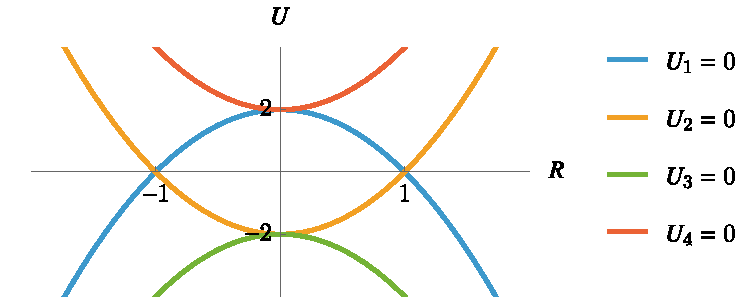
\includegraphics[width=.7\textwidth]{Delt0}
  \caption{The locus $\Delta(U, R) = 0$}
  \label{fig:Delt0}
\end{figure}

We can turn the quartic in \cref{eq:F0quartic} to cubic form by the following rational transformation
\begin{equation}
  X = \frac{a x + b}{c x + d}, \quad Y = \frac{a d - b c}{(c x + d)^2} y.
\end{equation}
The curve now looks like
\begin{equation}
  Y^2 = \frac{(a d - b c)^2}{(c x + d)^4} y^2 = f_4\qty(\frac{a x + b}{c x + d}).
\end{equation}
This implies,
\begin{equation}
  (a d - b c)^2 y^2 = f_4\qty(\frac{a x + b}{c x + d})(c x + d)^4 = c^4 f_4\qty(\frac{a}{c}) x^4 + f_3(x),
\end{equation}
where $f_3$ is a cubic polynomial in $x$ whose coefficient of $x^3$ is directly proportional to $f_4'(a/c)$. It follows that if we set $a/c$ to be a simple root of $f_4$ and $a d - b c = 1$ then we obtain the desired cubic form. We can then scale and translate so as to get the cubic in the usual Weierstrass form: $y^2 = 4 x^3 - g_2 x - g_3$.

Performing this procedure on the quartic in \cref{eq:F0quartic}, one gets
\begin{equation}
  \begin{aligned}
    g_2 &= \frac{1}{12} \left(16 R^8-8 R^4 \left(U^2+2\right)+\left(U^2-4\right)^2\right), \\
    g_3 &= \frac{1}{216} \left(4 R^4-U^2+4\right) \left(16 R^8-8 R^4 \left(U^2+5\right)+\left(U^2-4\right)^2\right).
  \end{aligned}
\end{equation}
We also find the $j$-invariant defined as $j = \frac{g_2^3}{g_2^3 - g_3^2}$,
\begin{equation}
  j = \frac{\left(16 R^8-8 R^4 \left(U^2+2\right)+\left(U^2-4\right)^2\right)^3}{R^8 \left(16 R^8-8 R^4 \left(U^2+4\right)+\left(U^2-4\right)^2\right)}.
\end{equation}

\subsection{Periods as double Laurent series}
From the GLSM charges defining the toric geometry, 
\begin{equation}
    \begin{array}{ccc|cc} 
    0 & 0 & 1 & -2 & -2 \\
    1 & 0 & 1 & 1 & 0 \\
    0 & -1 & 1 & 0 &1 \\
   -1 & 0 & 1 & 1 & 0 \\
   0  & 1 & 1 & 0 & 1 \\
   \end{array}
\end{equation}


we see that the periods of the mirror curve are given by the double sum
\begin{equation}
  \begin{aligned}
  \omega_1 =& \sum_{k,\ell\geq 0} \frac{(2k+2\ell)!}{(k!)^2 (\ell!)^2} z^{k+\ell} \lambda^{\ell} = F_4\qty(\tfrac12, 1; 1, 1; 4 z, 4 z \lambda)  \\
  \omega_2 =& (2\log z+ \log\lambda) \omega_1 - 2  
  \sum_{k+\ell>0} \frac{(2k+2\ell)!}{(k!)^2 (\ell!)^2} 
  \left( H_k + H_\ell - 2 H_{2k+2\ell} \right) 
  z^{k+\ell} \lambda^{\ell}
  \end{aligned}
\end{equation} 
where $F_4$ is the Appell hypergeometric series, and $H_n=\sum_{k=1}^n (1/k)$ are the harmonic numbers. 
For $\lambda=1$, we recover \cite[A.39]{LeFloch:2024cwl}, 
\begin{equation}
\omega_1 = {}_2F_1(\tfrac12,\tfrac12;1;16 z), \quad 
\omega_2 = -2\pi\  {}_2F_1(\tfrac12,\tfrac12;1;1-16 z),
\end{equation} 
Similarly, for $\lambda=-1$, we recover \cite[A.46]{LeFloch:2024cwl}, 
\begin{equation}
\omega_1 = {}_2F_1(\tfrac14,\tfrac34;1;-64z^2), \quad 
\omega_2 = -\pi \sqrt2\  {}_2F_1(\tfrac14,\tfrac34;1;1+64 z^2),
\end{equation} 
The CY periods satisfy $z\partial_z \varpi_2=\omega_1, z\partial_z \varpi_3=\omega_2$.
Hence they are obtained by integrating once with respect to $z$,
\begin{equation}
      \begin{aligned}
  \varpi_2 =& \log z + 
  2 \sum_{k+\ell>0} \frac{(2k+2\ell-1)!}{(k!)^2 (\ell!)^2} z^{k+\ell} \lambda^{\ell} \\
  \varpi_3 =& -\log^2 z 
  +  \left( 2\log z + \log\lambda\right) \varpi_2
   - 2  
  \sum_{k+\ell>0} \frac{(2k+2\ell)!}{(k!)^2 (\ell!)^2 (k+\ell)} 
  \left( H_k + H_\ell - 2 H_{2k+2\ell} + \frac{1}{k+\ell} \right) 
  z^{k+\ell} \lambda^{\ell}
  \end{aligned}
\end{equation}

\subsection{Kerr-Doran formula for the conifold period}

In \cite{kerr2008}, a formula is provided for periods of nodal curves in toric ambient spaces.
Here we check that this formula reproduces the result for the period at the conifold point 
derived in [A.84,A.107]\cite{LeFloch:2024cwl},
\begin{equation}
\begin{aligned}
T(\tau=0,m)= &  \frac{2}{\pi^2} \left( \Li_2( \I e^{\I\pi m/2} ) -  \Li_2(- \I e^{\I\pi m/2} )
\right)\\
T(\tau=\tfrac12,m)= &  \frac{2}{\pi^2} \left( \Li_2( e^{\I\pi m/2} ) -  \Li_2(- e^{\I\pi m/2} )
\right)\\
\end{aligned}
\end{equation}
where $R=e^{\I\pi m/2}$, such that $R^4=\lambda=e^{2\pi\I m}$. 

\subsubsection{Rational parametrization of the nodal curve}

As shown in \cref{eq:delt0sol}, the curve in \cref{eq:F0quartic} develops four distinct branches of nodes. These correspond to points in parameter space where the elliptic curve degenerates. Following the procedure outlined in \cite{kerr2008}, we rationally parametrize each nodal curve using a parameter $z$, such that the limits $z \to 0$ and $z \to \infty$ map to the node of the curve.

The quartic polynomial in \cref{eq:F0quartic} takes the following forms along the four branches, each associated with a corresponding node:
\begin{equation}
  \begin{aligned}
    U_1 &= 2 - 2R^2, &\qquad f_4(X) = (X+1)^2 \left(X^2 + \qty(2-4 R^2) X+1\right), && X_0 = -1, \\
    U_2 &= -2 + 2R^2, &\qquad f_4(X) = (X-1)^2 \left(X^2 + \qty(4 R^2-2) X+1\right), && X_0 = 1, \\
    U_3 &= -2 - 2R^2, &\qquad f_4(X) = (X-1)^2 \left(X^2+ \qty(-4 R^2-2) X+1\right), && X_0 = 1, \\
    U_4 &= 2 + 2 R^2, &\qquad f_4(X) = (X+1)^2 \left(X^2+\qty(4 R^2+2) X+1\right), && X_0 = -1.
  \end{aligned}
\end{equation}

To obtain a rational parametrization for the first branch ($U_1$), it suffices to find a rational expression for $X$ such that $\left(X^2 + \qty(2-4 R^2) X+1\right)$ becomes a perfect square. One convenient choice is
\begin{equation}
  X = \frac{2 \left(-2 R^2-t+1\right)}{t^2-1},
  \qquad
  \Rightarrow \qquad
  \left(X^2 + \qty(2-4 R^2) X+1\right) = 
  \qty(\frac{\left(4 R^2-2\right) t+t^2+1}{t^2-1})^2.
\end{equation}
The remaining parametrizations follow from the transformations $R^2 \to -R^2$ and $X \to -X$:
\begin{equation}
\begin{aligned}
  X_1 &= \frac{2 \left(-2 R^2-t+1\right)}{t^2-1}, &\quad
  Y_1 = \frac{-16 R^4 t+4 R^2 (t-1)^3+(t-1)^4}{\left(t^2-1\right)^2}, \\
  X_2 &= -\frac{2 \left(-2 R^2-t+1\right)}{t^2-1}, &\quad
  Y_2 = \frac{-16 R^4 t+4 R^2 (t-1)^3+(t-1)^4}{\left(t^2-1\right)^2}, \\
  X_3 &= -\frac{2 \left(2 R^2-t+1\right)}{t^2-1}, &\quad
  Y_3 = \frac{-16 R^4 t-4 R^2 (t-1)^3+(t-1)^4}{\left(t^2-1\right)^2}, \\
  X_4 &= \frac{2 \left(2 R^2-t+1\right)}{t^2-1}, &\quad
  Y_4 = \frac{-16 R^4 t-4 R^2 (t-1)^3+(t-1)^4}{\left(t^2-1\right)^2}.
\end{aligned}
\end{equation}
Each pair $(X_i, Y_i)$ satisfies \cref{eq:F0quartic} for the corresponding value of $U_i$.

Returning to the original toric coordinates $(X, w)$, the parametrizations become
\begin{equation}
  \begin{aligned}
  w_1 &= \frac{(t-1) \left(2 R^2+t-1\right)}{2 R^2 (t+1)}, \quad
  w_2 = -\frac{(t-1) \left(2 R^2+t-1\right)}{2 R^2 (t+1)}, \\
  w_3 &= \frac{(t-1) \left(2 R^2-t+1\right)}{2 R^2 (t+1)}, \quad
  w_4 = -\frac{(t-1) \left(2 R^2-t+1\right)}{2 R^2 (t+1)}.
  \end{aligned}
\end{equation}

This yields a rational parametrization of the nodal curve in toric coordinates, though the node still lies at a finite distance rather than at $0$ or $\infty$. To remedy this, we perform one final change of variables. For $U_1$, the node at $X_0 = -1$ corresponds to $t = 1 \pm 2R$, so we define
\begin{equation}
  z = \frac{t - (1-2R)}{t - (1+2R)},
\end{equation}
similarly, for $U_2$. For $U_3$ and $U_4$, the node corresponds to $t = 1 \pm 2 \ii R$, so we define
\begin{equation}
  z = \frac{t - (1-2\ii R)}{t - (1+2\ii R)}.
\end{equation}
Therefore, for each branch we get $X$ and $w$ in the $z$-parametrization:
\begin{equation}\label{eq:F0rationalparam}
  \begin{aligned}
    X_1 &= -\frac{(z-1) (R (z-1)+z+1)}{(z+1) (R z+R+z-1)}, &\quad
    w_1 = \frac{(z+1) (R (z-1)+z+1)}{(z-1) (R z+R+z-1)}, \\
    X_2 &= \frac{(z-1) (R (z-1)+z+1)}{(z+1) (R z+R+z-1)}, &\quad
    w_2 = -\frac{(z+1) (R (z-1)+z+1)}{(z-1) (R z+R+z-1)}, \\
    X_3 &= \frac{(z-1) (R (z-1)+i (z+1))}{(z+1) (R (z+1)+i (z-1))}, &\quad
    w_3 = \frac{(z+1) (R (z-1)+i (z+1))}{(z-1) (R (z+1)+i (z-1))}, \\
    X_4 &= -\frac{(z-1) (R (z-1)+i (z+1))}{(z+1) (R (z+1)+i (z-1))}, &\quad
    w_4 = -\frac{(z+1) (R (z-1)+i (z+1))}{(z-1) (R (z+1)+i (z-1))}.
  \end{aligned}
\end{equation}

\subsubsection{Conifold period for a real curve}

Applying the method of \cite[Section~4.2]{kerr2008}, we find for the first branch the exponents and roots of the linear factors (with $i=1$, $j = 1,\dots,4$):
\begin{equation}
  \begin{aligned}
    (d_j) &= (1, 1, -1, -1), &\quad (\alpha_j) = \qty(1,\frac{R-1}{R+1},-1,\frac{1-R}{R+1}), \\
    (e_j) &= (1, 1, -1, -1), &\quad (\beta_j) = \qty(-1,\frac{R-1}{R+1},1,\frac{1-R}{R+1}).
  \end{aligned}
\end{equation}

The (imaginary part of the) non-vanishing period at the conifold point is then
\begin{equation}
  \mathcal{P}(R) = \frac{1}{2\pi} \sum_{j, k} d_j e_k D_2\qty(\frac{\alpha_j}{\beta_k}),
\end{equation}
where $D_2(z)$ is the Bloch--Wigner function,
\begin{equation}
  D_2(z) = \Im\!\qty(\operatorname{Li}_2(z)) + \arg(1-z)\,\log\abs{z},
\end{equation}
and $\operatorname{Li}_2(z)$ denotes the ordinary dilogarithm \cite{zagier:dilogarithm}.

We thus find, up to an overall sign,
\begin{equation}
  \mathcal{P}(R) = \frac{1}{\pi} \qty[-D_2\!\left(\frac{R+1}{1-R}\right)
  + D_2\!\left(\frac{R+1}{R-1}\right)
  + D_2\!\left(\frac{1-R}{R+1}\right)
  - D_2\!\left(\frac{R-1}{R+1}\right)].
\end{equation}
Using the Bloch--Wigner identities \cite[Eq.~(3)]{zagier:dilogarithm},
\begin{equation}
  D_2(z) = D_2\!\qty(1-\frac{1}{z}) = D_2\!\qty(\frac{1}{1-z})
  = -D_2\!\qty(\frac{1}{z}) = -D_2(1-z)
  = -D_2\!\qty(\frac{-z}{1-z}),
\end{equation}
we note that
\begin{equation}
  D_2\!\qty(\frac{1-R}{1+R}) = -D_2\!\left(\frac{R+1}{1-R}\right),
  \qquad
  D_2\!\left(\frac{R-1}{R+1}\right) = -D_2\!\left(\frac{R+1}{R-1}\right),
\end{equation}
so that
\begin{equation}\label{eq:realPeriod}
  \mathcal{P}(R) = \frac{2}{\pi}
  \qty[D_2\!\left(\frac{R+1}{R-1}\right)
  - D_2\!\left(\frac{R+1}{1-R}\right)].
\end{equation}
We now use the five-term relation for the Bloch-Wigner,
\begin{equation}
  D_2\left(\frac{1-x}{1-x y}\right)+D_2\left(\frac{1-y}{1-x y}\right)+D_2(1-x y)+D_2(x)+D_2(y) = 0,
\end{equation}
with $x = R$, $y = -1$, to simplify the imaginary part of the period to the simple expression
\begin{equation}
  \mathcal{P}(R) = \frac{2}{\pi } \bigl[D_2(-R)-D_2(R)\bigr].
\end{equation}
Since $D_2(\bar{z}) = -D_2(z)$, it follows that
\begin{equation}
  \mathcal{P}(R) = 0 \qquad \text{for real } R.
\end{equation}

Repeating the analysis for $U_2$ yields identical exponents and roots, and thus the same result. For $U_3$ and $U_4$, the change of variables is $t = \frac{-2 \ii R (z+1)+z-1}{z-1}$, giving
\begin{equation}
  \begin{aligned}
    (d_j) &= (1, 1, -1, -1), &\quad
    (\alpha_j) = \qty(1,\frac{R-\ii}{R+\ii},-1,\frac{\ii-R}{R+\ii}), \\
    (e_j) &= (1, 1, -1, -1), &\quad
    (\beta_j) = \qty(-1,\frac{R-\ii}{R+\ii},1,\frac{\ii-R}{R+\ii}).
  \end{aligned}
\end{equation}
Hence,
\begin{equation}\label{eq:imagPeriod}
  \begin{aligned}
    \mathcal{P}(R)
    &= \frac{1}{\pi}\qty[-D_2\!\left(\frac{R+i}{-R+i}\right)
      + D_2\!\left(\frac{R+i}{R-i}\right)
      + D_2\!\left(\frac{-R+i}{R+i}\right)
      - D_2\!\left(\frac{R-i}{R+i}\right)] \\
    &= \frac{2}{\pi} \qty[D_2\!\left(\frac{-R+i}{R+i}\right)
      - D_2\!\left(\frac{R-i}{R+i}\right)].
  \end{aligned}
\end{equation}
Applying the five term relation gives us
\begin{equation}
  \mathcal{\tilde{P}}(R) = \frac{2}{\pi} \bigl[D_2(\ii R)-D_2(-\ii R)\bigr]
\end{equation}
And this time we see that \bp{But the formula should not apply}
\begin{equation}
  \mathcal{P}(R) = 0 \qquad \text{for imaginary } R.
\end{equation}

% We want to now understand how (and/or if) the formulas \cref{eq:realPeriod,eq:imagPeriod} reproduce the formulas for the 'quantum volumes' in \cite[eq. (A.85) and eq. (A.107)]{LeFloch:2024cwl} which we copy below for reference after identifying $\lambda = e^{2\pi\ii m}$ and from the parametrization of the mirror curve, we identify $R = \lambda^\frac{1}{4} = e^{\ii \pi m/2}$,
% \begin{align}
%   \mathcal{V}(R) &= \frac{2 \ii}{\pi^2} \qty(\Li_2(-\ii R) - \Li_2(\ii R)), \\
%   \tilde{\mathcal{V}}(R) &= \frac{2 \ii}{\pi^2} \qty(\Li_2(-R) - \Li_2(R)) = \mathcal{V}(-\ii R).
% \end{align}
% Since $D_2$ is the imaginary part of $\Li_2$, we must look at the full non-vanishing period to make this identification. 

\subsubsection{Conifold period for general moduli}
In fact, apart from the imaginary part of the period, \cite[eq. (4.12)]{kerr2008} also gives a formula for the full non-vanishing period at the conifold points, even when the curve is not real:
\begin{equation}\label{eq:fullperiodkerrdonan}
\begin{aligned}
  \mathcal{Q} &= \frac{1}{2\pi} \sum_{j, k} d_j e_k \qty[ \Li_2\qty(\frac{\alpha_j}{\beta_k}) + \qty(\log \alpha_j - \log \beta_k) \log(1 - \frac{\alpha_j}{\beta_k}) ] \\
  &\quad -\frac{1}{2\pi} \log y(0) \qty(\log x(0) - \log x(\infty))
  + \log y(0) \sum_j d_j \log \alpha_j \\
  &\quad - \log x(\infty) \sum_k e_k \log \beta_k.
\end{aligned}
\end{equation}
where as before, $x(z)$ and $y(z)$ are rational parametrizations of the nodal curve in the original toric coordinates and the node corresponds to $z \to 0, \infty$.
From now on, we work with the branches $U_1$ and $U_2$ but all the results can be generalized to $U_3$ and $U_4$ by taking $R \to \ii R$.
Evaluating \cref{eq:fullperiodkerrdonan} for the parametrization in \cref{eq:F0rationalparam}, we find the following after assuming $\Im R > 0$ and simplifying logs
\begin{equation}
  \begin{aligned}
    \mathcal{Q} &= \frac{1}{\pi} \qty(\Li_2\left(\frac{-R-1}{R-1}\right)-\Li_2\left(\frac{R+1}{R-1}\right)-\Li_2\left(\frac{1-R}{R+1}\right)+\Li_2\left(\frac{R-1}{R+1}\right)) \\
    &\quad -\frac{2}{\pi} \log (R) \log (R-1)+i  \log (R-1)+2 i  \log (R)\\
    &\quad +\frac{2}{\pi} \log (R) \log (R+1)-i  \log (R+1).
    \end{aligned}
\end{equation}

This expression can be simplified further thanks to various identities of the dilogarithm. We use in particular the following identities \cite{zagier:dilogarithm}
\begin{align}
  \Li_2\qty(\frac{1}{z}) &= -\Li_2(z) - \frac{\pi^2}{6} - \frac{1}{2}\log(-z)^2, \label{eq:Li2Inversion}\\
  \Li_2\qty(1-z) &= -\Li_2(z) + \frac{\pi^2}{6} - \log(z) \log(1-z). \label{eq:Li2Reflection}
\end{align}
We also have the so-called \textit{five term relation},
\begin{equation}
  \begin{aligned}
    &\Li_2(x)+\Li_2(y)+\Li_2\left(\frac{x-1}{x y-1}\right)+\Li_2\left(\frac{y-1}{x y-1}\right)+\Li_2(1-x y) \\
    &= \frac{\pi ^2}{2} - \log (1-x) \log (x)- \log (1-y) \log (y) -\log \left(\frac{1-x}{1-x y}\right) \log \left(\frac{1-y}{1-x y}\right),
  \end{aligned}
\end{equation}
which only holds near the viscinity of $x, y \in (0, 1)$ due to branch cuts. However, it is easy to find a generalized version of this identify for the domain we are interested in by starting with the identity in it's twice differentiated form (where it reduces to a trivial algebraic identity) and integrating twice and fixing the integration constants.

Using the inversion identity \cref{eq:Li2Inversion}, we get
\begin{equation}
  \begin{aligned}
  \mathcal{Q} &= -\frac{\pi}{2} -\frac{2}{\pi} \qty[\Li_2\left(\frac{1-R}{R+1}\right)- \Li_2\left(\frac{R-1}{R+1}\right) -  \log \left(\frac{1-R}{R+1}\right) \log (R)].
  \end{aligned}
\end{equation}
We now invoke the five term relation with $(x, y) = (R, -1)$ and correct it with the procedure explained. After applying the reflection identity to some of the arguments \cref{eq:Li2Reflection} and noting that $\Li_2(-1) = \frac{-\pi^2}{12}$, the identity reads simply
\begin{equation}
  -\Li_2(-R)+\Li_2(R)+\Li_2\left(\frac{1-R}{R+1}\right)-\Li_2\left(\frac{R-1}{R+1}\right)
  = \frac{\pi ^2}{4}-\log (R) \log \left(\frac{1-R}{R+1}\right).
\end{equation}
Applying this to $Q$, we get our final expression
\begin{equation}
  \mathcal{Q} = - \pi - \frac{2}{\pi} \qty[\Li_2(-R)- \Li_2(R)].
\end{equation}


\section{Local \texorpdfstring{$\mathbb{F}_1$}{F1}}


\subsection{Nagell's algorithm for the mirror curve}
We start from the equation of the local mirror of $\mathbb{F}_1$ defined as the elliptic curve,
\begin{equation}\label{eq:F1mirror}
  x + y + \frac{1}{x y} + \frac{m}{x} = \frac{1}{u},
\end{equation}
where $m$ and $u$ are a priori free complex parameters. After multiplying by $x y$, we have
\begin{equation}
  f(x, y) = x^2 y + x y^2 - \frac{x y}{u} + m y + 1 = 0.
\end{equation}
We can eliminate the constant term by shifting $y \to y - \frac{1}{m}$,
\begin{equation}
  f(x, y) = x^2 y + x y^2 - \frac{x^2}{m} - \frac{(2u + m) x y}{u m} + m y + \frac{(m + u)x}{m^2 u}.
\end{equation}
We perform a series of affine transformations on $x$ and $y$ known as Nagell's algorithm as described in \cite{ConnellHandbook} to bring the curve into Weierstrass form. Note that in order for the curve to be elliptic, $m$ and $u$ cannot vanish simultaneously. Since we would be interested in the $m \to 0$ limit (Local $\mathbb{P}^2$), we switch $x \leftrightarrow y$ and assume generically that $m + u \neq 0$. We thus have
\begin{equation}
  f(x, y) = x^2 y + x y^2 - \frac{y^2}{m} - \frac{(2u + m) x y}{u m} + m x + \frac{(m + u)y}{m^2 u}.
\end{equation}
Let us homogenize by writing $x = X/Z$, $y = X/Z$ and clearing denominators. We get,
\begin{equation}
  F(X, Y, Z) = F_3(X, Y) + F_2(X, Y) Z + F_1(X, Y) Z^2.
\end{equation}
where
\begin{align}
  F_3 &= X^2 Y + X Y^2, \\
  F_2 &= -\frac{(2u + m)}{u m} X Y - \frac{Y^2}{m}, \\
  F_1 &= m X + \frac{(m+u)}{m^2 u}  Y.
\end{align}
Note that the point $P = [0, 0, 1]$ is rational by construction (after eliminating the constant term). The tangent at $P$ is given by $F_1 = m X + \frac{(m+u)}{m^2 u} Y = 0$ and meets the curve at another point $Q$. We also define $e_i = F_i\qty(\frac{(m+u)}{m^2 u}, -m)$ ($e_1 = 0$ by definition) ---
\begin{align}
  e_2 &= \frac{2}{m^2}+\frac{3}{m u}-m+\frac{1}{u^2}, \\
  e_3 &= \frac{(m+u) \left(u-\frac{m+u}{m^3}\right)}{u^2}.
\end{align}
The coordinates of $Q$ are given by
\begin{equation}
  \begin{split}
    Q = \Big[& \frac{(m+u) \left(m^3 u^2-m^2-3 m u-2 u^2\right)}{m^4 u^3}, \\
    &-m^2+\frac{m}{u^2}+\frac{2}{m}+\frac{3}{u},\quad \frac{(m+u) \left(u-\frac{m+u}{m^3}\right)}{u^2} \Big].
  \end{split}
\end{equation}
For the curve to be elliptic, $e_2$ and $e_3$ cannot vanish simultaneously which is true provided $m$ and $u$ don't vanish simultaneously. On the real section of the $m$ -- $u$ plane, these conditions are plotted in \cref{fig:e2e3Vanish}.

\begin{figure}[htbp]
  \centering
  % first subfigure
  \begin{subfigure}[t]{0.4\textwidth}
    \centering
    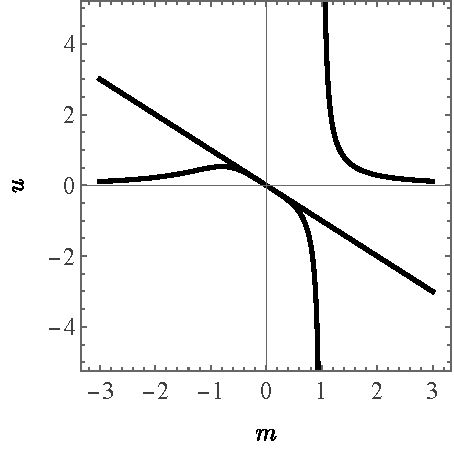
\includegraphics[width=\linewidth]{figures/e3Vanish}
    \caption{$e_3 = 0$}
    \label{fig:e3Vanish}
  \end{subfigure}
  \hfill
  % second subfigure
  \begin{subfigure}[t]{0.4\textwidth}
    \centering
    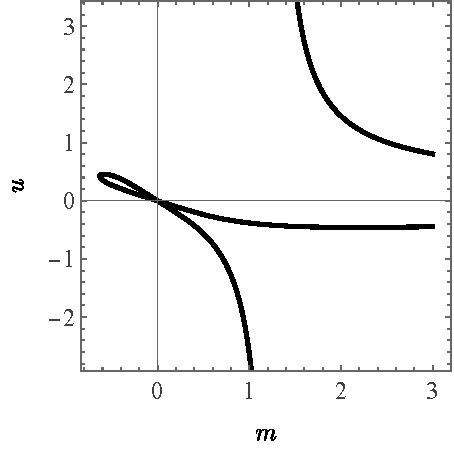
\includegraphics[width=\linewidth]{figures/e2Vanish}
    \caption{$e_2 = 0$}
    \label{fig:e2Vanish}
  \end{subfigure}

  \caption{The loci where $e_2$, $e_3$ vanish.}
  \label{fig:e2e3Vanish}
\end{figure}

Assuming generically that $e_3 \neq 0$, we make the coordinate change
\begin{align}
  X &= X' + \frac{m u \left(\frac{2}{m^2}+\frac{3}{m u}-m+\frac{1}{u^2}\right)}{m+u-m^3 u} Z' \\
  Y &= Y' - \frac{m^2 \left(m^3 \left(-u^2\right)+m^2+3 m u+2 u^2\right)}{(m+u) \left(m+u-m^3 u\right)} Z' \\
  Z &= Z'
\end{align}
which shifts $Q$ to the origin, $[X', Y', Z'] = [0, 0, 1]$. We now shift back to affine coordinates $x' = X'/Z'$, $y' = Y'/Z'$. The curve can now be written as
\begin{equation}
  f'(x', y') = f_3'(x', y') + f_2'(x', y') + f_1'(x', y')
\end{equation}
where
\begin{align}
  f_3' \ = \ & x'^2 y' + x' y'^2 \\
  f_2' \ = \ & \frac{(m+u)^2}{m u \left(m+u-m^3 u\right)} y'^2 + \qty(\frac{2 \left(m+u-m^3 u\right)}{m (m+u)}+\frac{1}{u}) x' y' \notag \\
  & + \frac{m^2 \left(-\left(m^3-2\right) u^2+m^2+3 m u\right)}{(m+u) \left(\left(m^3-1\right) u-m\right)} x'^2 \\
  f_1' \ = \ & \frac{(m+u) \left(2 m^6 u^2-m^5-5 m^4 u-4 m^3 u^2+m^2+2 m u+u^2\right)}{m^2 u \left(m+u-m^3 u\right)^2} y' \notag \\
  & + \frac{m}{u (m+u)^2 \left(m+u-m^3 u\right)^2} \bigl( -m^5-6 m^4 u+\left(m^3-15\right) m^3 u^2 \notag \\
  & \qquad -3 \left(m^6-3 m^3+4\right) m u^4+\left(6 m^3-19\right) m^2 u^3 \notag \\
  & \qquad +\left(m^9-3 m^6+4 m^3-3\right) u^5 \bigr) x'
\end{align}
We define $\phi_i = f_i'(1, t)$ and
\begin{equation}
  \begin{split}
    \delta &= \phi_2^2 - 4 \phi_1 \phi_3 \\
    &= \frac{(m+u)^4}{m^2 u^2 \left(m+u-m^3 u\right)^2} t^4 \\
    & \quad - \frac{2 (m+u) \left(-\left(5 m^3+1\right) u^2-m \left(m^3+2\right) u-m^2+2 m^2 \left(m^3-2\right) u^3\right)}{m u^2 \left(m+u-m^3 u\right)^2} t^3 \\
    & \quad + \frac{1}{u^2 \left(m+u-m^3 u\right)^2} \bigl( 2 m \left(2 m^3+1\right) u+m^2+2 m \left(-2 m^6+m^3+4\right) u^4 \\
    & \qquad +\left(m^6+18 m^3+1\right) u^2+2 m^2 \left(m^3+11\right) u^3 \bigr) t^2 \\
    & \quad + \frac{2 m}{u (m+u) \left(m+u-m^3 u\right)^2} \bigl( m^4+\left(m^3+4\right) m^3 u+2 \left(-m^6+m^3+1\right) u^4 \\
    & \qquad +\left(-3 m^6+7 m^3+6\right) m u^3+\left(6 m^3+7\right) m^2 u^2 \bigr) t \\
    & \quad + \frac{m^4 \left(-\left(m^3-2\right) u^2+m^2+3 m u\right)^2}{(m+u)^2 \left(m+u-m^3 u\right)^2}
  \end{split}
\end{equation}
Note that $\delta = 0$ whenever $t$ is the slope of a tangent to the curve that passes through $Q$, in particular for $t = -\frac{m^3 u}{m+u}$ (can be checked). We write $t = \frac{1}{\tau} -\frac{m^3 u}{m+u}$ and define $\rho = \tau^4 \delta$ which is a cubic in $\tau$
\begin{equation}
  \begin{split}
    \rho \ = \ &\frac{4 m \left(m+u-m^3 u\right)}{m+u} \tau^3 + \qty(8 m+\frac{1}{u^2}) \tau^2 + \frac{2 (m+u) \left(2 m^2 u^2+m+u\right)}{m u^2 \left(m+u-m^3 u\right)} \tau \\
    & + \frac{(m+u)^4}{m^2 u^2 \left(m+u-m^3 u\right)^2}.
  \end{split}
\end{equation}
Applying the final transformation,
\begin{align}
  \rho &= \frac{(m+u)^2}{m^2 \left(m+u-m^3 u\right)^2} V^2, \\
  \tau &= \frac{(m+u)}{m \left(m+u-m^3 u\right)} \bigl( U - \frac{1}{12} \qty(8 m+\frac{1}{u^2}) \bigr),
\end{align}
we obtain the final Weierstrass form,
\begin{equation}
  V^2 = 4 U^3 - g_2 U + g_3,
\end{equation}
with
\begin{align}\label{eq:F1g23Nagell}
  g_2 &= -\frac{4}{3} \qty(-16 m^2+\frac{8 m}{u^2}-\frac{1}{u^4}+\frac{24}{u}), \\
  g_3 &= -\frac{8}{27} \qty(-64 m^3+\frac{48 m^2}{u^2}-\frac{12 m}{u^4}+\frac{144 m}{u}+\frac{1}{u^6}-\frac{36}{u^3}+216).
\end{align}


\subsection{Periods as double Laurent series}
From the GLSM charges defining the toric geometry, 
\begin{equation}
    \begin{array}{ccc|cc} 
    0 & 0 & 1 & -2 & -1 \\
    1 & 0 & 1 & 1 & 0 \\
    -1 & -1 & 1 & 0 &1 \\
   -1 & 0 & 1 & 1 & -1 \\
   0  & 1 & 1 & 0 & 1 \\
   \end{array}
\end{equation}
we see that the A-period of the mirror curve is given by the double sum
\begin{equation}
  \begin{aligned}
  \omega_1 =& 
  \sum_{k,\ell\geq 0} \frac{(k+2\ell)!}{(k!)^2 (l!) (\ell-k)!} 
  (-u)^{-k-2\ell} \lambda^{\ell-k}  \\
  = &
  \sum_{k,\ell\geq 0} \frac{(3k+2\ell)!}{(k!)^2 (k+\ell)! (\ell!)} 
  (-u)^{-3k-2\ell} \lambda^{\ell} 
  \end{aligned}
\end{equation}
\rishi{where $z_1 = \frac{\lambda}{u^2}$, $z_2 = \frac{1}{u \lambda}$ are the standard complex structure parameters? \\
related to Marcos' parameters by $u_\text{here} = -\frac{1}{u_\text{Marcos}}$, $\lambda = m$?} \\
where in the second line we shifted $\ell\mapsto \ell+k$, observing that terms with $k>\ell$ do not contribute in the sum in the first line. Indeed, we check that $\omega_1$ is annihilated by the second order operator
\begin{equation}
\begin{aligned}
        \mathcal{D}
    =& (8 \lambda  u-9) \left(16 \lambda ^3+\lambda  u^4-u^3-8 \lambda ^2 u^2+36 \lambda  u-27\right) \theta_u^2 \\ &
     +(-729 + 1512 u \lambda - 
     u^4 \lambda - 936 u^2 \lambda^2 + 432 \lambda^3 + 
     128 u^3 \lambda^3 - 512 u \lambda^4) \theta_u 
      \\ &   
     -2 (-243 + 486 u \lambda - 282 u^2 \lambda^2 + 
     144 \lambda^3 + 32 u^3 \lambda^3 - 
     192 u \lambda^4) 
     \end{aligned}
\end{equation}\
such that $\mathcal{D}_3= u^{-3} \mathcal{D} \partial_u$. 
Using the Frobenius method, we find two logarithmic solutions
\begin{equation}
  \begin{aligned}
  \omega_2 =& (-\log u -\log\lambda) \omega_1 + 2  
  \sum_{-2\ell<k\leq \ell} 
  \frac{(k+2\ell)!}{(k!)^2 (k)! (\ell-k)!} 
  \left( H_{2\ell+k} + H_{\ell-k} - 2 H_{k} \right) 
 (-u)^{-k-2\ell} \lambda^{\ell-k} \\ & 
 + \sum_{0\leq \ell<k} (-1)^{\ell}  \frac{\Gamma(k-\ell) (k+2\ell)!}{\ell!\, (k!)^2} 
 u^{-k-2\ell} \lambda^{\ell} 
 \\
 \omega'_2 =& (-2\log u +\log\lambda) \omega_1 + 2  
  \sum_{-2\ell<k\leq \ell} 
  \frac{(k+2\ell)!}{(k!)^2 (k)! (\ell-k)!} 
  \left( 2H_{2\ell+k} - H_{\ell-k} -  H_{\ell} \right) 
 (-u)^{-k-2\ell} \lambda^{\ell-k}\\ & 
 - \sum_{0\leq \ell<k} (-1)^{\ell}  \frac{\Gamma(k-\ell) (k+2\ell)!}{\ell!\, (k!)^2} 
 u^{-k-2\ell} \lambda^{\ell} 
  \end{aligned}
\end{equation} 
where $H_n=\sum_{k=1}^n (1/k)$ are the harmonic numbers. In fact, only the linear combination $2\omega_2+3\omega'_2$ is annihilated by $\mathcal{D}$, while
$\omega_2$ and $\omega'_2$ satisfy it with a source term proportional to $9\lambda u^4 +96 \lambda^3 u^3$. 

The CY periods satisfy $u\partial_u \varpi_2=\omega_1, u\partial_u \varpi_3=\frac14(2\omega_2+3\omega'_2)$.
Hence they are obtained by integrating once with respect to $u$,
\begin{equation}
      \begin{aligned}
  \varpi_2 =& -\log u + 
  \sum_{3k+2\ell>0} \frac{(3k+2\ell-1)!}{(k!)^2 (\ell!)(k+\ell)!} 
  (-u)^{-3k-2\ell} \lambda^{\ell}  \\
  \varpi_3 =& \log^2 u + (2\log u - \frac14 \log \lambda) \varpi_2 + \frac18 \log^2\lambda 
  \\ &
-2  \sum_{-2\ell<k\leq \ell} 
  \frac{(k+2\ell-1)!}{(k!)^2 (k)! (\ell-k)!} 
  \left( 2H_{2\ell+k} - H_{\ell-k} -  H_{\ell} \right) 
 (-u)^{-k-2\ell} \lambda^{\ell-k}\\ & 
 + \sum_{0\leq \ell<k} (-1)^{\ell}  \frac{\Gamma(k-\ell) (k+2\ell-1)!}{\ell!\, (k!)^2} 
 u^{-k-2\ell} \lambda^{\ell} 
 -2 \sum_{k+2\ell>0}  \frac{(k+2\ell-1)!}{(k+2\ell)(k!)^2 (k)! (\ell-k)!} u^{-k-2\ell} \lambda^{\ell} 
  \end{aligned}
\end{equation}

\paragraph{Streamlined expressions for the large volume expansion}

\begin{align}
  m &= \frac{1}{3} X^{(1)}, \\
  t &= X^{(2)} + \frac{1}{3} X^{(1)}, \\
  t_D &= 4 X^{(3)} + \frac{1}{6} X^{(0)},
\end{align}
where
\begin{align}
  X^{(0)} &= 1, \qquad X^{(1)} = \frac{1}{2\pi \ii} \log \ell, \\
  X^{(2)} &= \frac{1}{2\pi\ii} \big(\log \ur + \sigma_1(\ur, \ell) \big), \\
  X^{(3)} &= \begin{aligned}[t]
    \frac{1}{(2\pi\ii)^2} & \Bigl[ (\log\ur)^2 + \frac34 \log \ell \log \ur + \frac18 (\log \ell)^2 
    + \Big( 2 \log \ur + \frac34 \log \ell \Big)\sigma_1(\ur, \ell) \\
    &\quad + \sigma_2(\ur, \ell)  \Bigr],
  \end{aligned}
\end{align}
are the solutions of the Picard-Fuchs equations in standard Frobenius basis and $\sigma_i$ are the following series
\begin{align}
  \sigma_1 &= \begin{aligned}[t]
    &\sum_{n=2}^{\infty} (n-1)! \Big( \sum_{r = \ceil{n/3}}^{\floor{n/2}} \frac{\ell^r}{r! (n-2r)!^2 (3r-n)!} \Big) \ur^n \\
    &= \ell \,\ur^{2} + 2\ell \,\ur^{3} + \frac{3}{2}\ell^{2}\ur^{4} + 12\ell^{2}\ur^{5} + O(\ur^{6}),
  \end{aligned} \\
  \sigma_2 &= \begin{aligned}[t]
    &-\sum_{n=1}^{\infty} \frac{(n-1)!}{4}\Bigg[
    \sum_{r=0}^{\left\lfloor (n-1)/3 \right\rfloor}
    \frac{(-1)^{\,n-r}(n-3r-1)!}{r!\,(n-2r)!^2}\,\ell^r
    \\
    &\qquad\qquad\quad
    +\sum_{r=\left\lceil n/3 \right\rceil}^{\left\lfloor n/2 \right\rfloor}
    \frac{\ell^r}{r!\,(n-2r)!^2\,(3r-n)!}
    \left(
    4H_{n-2r}+3H_r+H_{3r-n}-8H_{n-1}
    \right)
    \Bigg] \ur^n \\
    &= \frac{\ur}{4}
      +\left(\ell-\frac{1}{16}\right)\ur^{2}
      +\left(\frac{1}{36}+\frac{5\ell}{2}\right)\ur^{3}
      +\frac{-1+24\ell+208\ell^{2}}{64}\,\ur^{4}
      +O(\ur^{5}).
  \end{aligned}
\end{align}

It follows that for $\tau = \frac{\partial_\ur T_D}{\partial_\ur T}$,
\begin{equation}
  \begin{aligned}
    \log q = 2 \pi \ii \, \tau &= \bigl(8 \log \ur + 3 \log \ell\bigr) + \frac{4 \ur \sigma_2' + 8 \sigma_1}{1+\ur \sigma_1'} \\
    &= \bigl(8\log \ur + 3\log \ell\bigr) + \ur + \frac{1}{2}(-1 + 32\ell)\ur^2 + \frac{1}{3}(1 + 132\ell)\ur^3 \\
    &\qquad + \frac{1}{4}(-1 + 4\ell + 128\ell^2)\ur^4 + \frac{1}{5}(1 - 5\ell + 1680\ell^2)\ur^5 + O(\ur^6).
  \end{aligned}
\end{equation}



\subsection{Rational change of coordinates and the Kerr-Doran prescription}

\subsubsection{Older analysis in the \texorpdfstring{$(m, u)$}{(m, u)} coordinates}

Nagell's algorithm provides a systematic procedure to convert the mirror curve of local $\mathbb{F}_1$ into Weierstrass form, but it does so at the price of introducing a transcendental change of variables. A significantly simpler rational transformation, originally presented in \cite{Marino:LocalF1Notes}, is given by
\begin{equation}
  x = \frac{36 u^2 (m+3 u)+6 X+\sqrt{2}\, Y-9}{6 u \left(12 m u^2+2 X-3\right)}, 
  \qquad 
  y = \frac{36 u^2}{-12 m u^2-2 X+3}.
\end{equation}
In these coordinates the mirror curve \cref{eq:F1mirror} assumes Weierstrass form,
\begin{equation}
  Y^2 = 4X^3 - g_2 X - g_3,
\end{equation}
with
\begin{equation}\label{eq:g2g3mirrorcurve}
\begin{aligned}
  g_2 &= 27\left( 16 m^2 u^4 - 8 m u^2 - 24 u^3 + 1 \right), \\
  g_3 &= 27\left( 64 m^3 u^6 - 48 m^2 u^4 - 144 m u^5 + 12 m u^2 - 216 u^6 + 36 u^3 - 1 \right).
\end{aligned}
\end{equation}
These expressions agree with \cref{eq:F1g23Nagell} up to an overall normalization, which can be absorbed by rescaling $X$ and $Y$. The discriminant takes the form
\begin{equation}\label{eq:deltamirrorcurve}
  \Delta \propto u^8\, \delta(u,m),
  \qquad
  \delta(u,m) = 16 m^3 u^4 - 8 m^2 u^2 - 36 m u^3 + m - 27 u^4 + u,
\end{equation}
showing that for fixed $m$ the curve generically develops four nodal degenerations corresponding to the roots of $\delta(u,m)=0$. Among these solutions we single out the branch $u_{*}(m)$ of smallest absolute value; this root is the one governing, for example, the convergence of the large-radius expansion of the periods, and will therefore play a distinguished role in the analysis.

To treat all nodal branches uniformly we follow the formalism of \cite{Marino:LocalF1Notes}. At the nodal locus the curve can be written as
\begin{equation}\label{eq:nodalcurve}
  Y^2 = 4 (X - X_0)^2 (X - X_1).
\end{equation}
Eliminating the $X^2$ term enforces $X_1 = -2 X_0$. Matching coefficients with the Weierstrass form then yields
\begin{equation}
  X_0 = -\frac{3 g_3}{2 g_2},
\end{equation}
evaluated on the discriminant locus $\delta(u,m)=0$. A convenient rational parametrization of \cref{eq:nodalcurve} is
\begin{equation}\label{eq:nodalcurveparamorig}
  X = \frac{1}{2}\left(t^2 - 4 X_0\right),
  \qquad
  Y = \frac{t\left(t^2 - 6 X_0\right)}{\sqrt{2}}.
\end{equation}
Expressed back in the original toric coordinates, this leads to
\begin{equation}
\begin{aligned}
  x &= \frac{36 u^2 (m+3 u)+3 (t^2 - 4 X_0) + t(t^2 - 6 X_0) - 9}{6 u \left(12 m u^2 + t^2 - 4 X_0 - 3\right)}, \\
  y &= \frac{36 u^2}{-12 m u^2 - t^2 + 4 X_0 + 3}.
\end{aligned}
\end{equation}
Introducing the notation
\begin{equation}
  t_1^2 = -12 m u^2 + 4 X_0 + 3,
\end{equation}
the denominators become $t^2 - t_1^2 = (t - t_1)(t + t_1)$. On the discriminant locus one may verify that the numerator of $x$ factorizes as
\begin{equation}
  36 u^2 (m+3 u)+3(t^2 - 4 X_0) + t(t^2 - 6 X_0) - 9 
  = (t - t_1)^2 (t + 2 t_1 + 3),
\end{equation}
which leads to the one-parameter family
\begin{equation}\label{eq:tparam}
  x = \frac{(t - t_1)(t + 2 t_1 + 3)}{6 u (t + t_1)},
  \qquad
  y = -\frac{36 u^2}{t^2 - t_1^2}.
\end{equation}

To apply the Kerr–Doran prescription we shift the nodes to $0$ and $\infty$. From \cref{eq:nodalcurveparamorig} the node occurs at $t=\pm\sqrt{6X_0}$, leading to the coordinate
\begin{equation}
  z = \frac{t - \sqrt{6 X_0}}{t + \sqrt{6 X_0}}.
\end{equation}
In terms of $z$, the parametrization \cref{eq:tparam} takes the form
\begin{equation}
  x = \alpha\, \frac{(z-a)(z-b)}{(z-c)(z-1)},
  \qquad
  y = \beta\, \frac{(z-1)^2}{(z-b)(z-c)},
\end{equation}
where
\begin{equation}\label{eq:nodalcurveparams}
\begin{gathered}
  b = \frac{t_1 - \sqrt{6X_0}}{t_1 + \sqrt{6X_0}},
  \qquad
  a = \frac{3 + 2t_1 + \sqrt{6X_0}}{3 + 2t_1 - \sqrt{6X_0}} = \frac{1}{b^2},
  \qquad
  c = \frac{t_1 + \sqrt{6X_0}}{t_1 - \sqrt{6X_0}} = \frac{1}{b},
  \\
  \alpha = \frac{t_1 + 3}{6 u}
  = \left(\sqrt{b} + \frac{1}{\sqrt{b}}\right)^{-\tfrac{4}{3}},
  \qquad
  \beta = -\frac{18 u^2}{t_1^2+3 t_1} = \left(\sqrt{b} + \frac{1}{\sqrt{b}}\right)^{\tfrac{2}{3}}.
\end{gathered}
\end{equation}

Using the general expression for the imaginary part of the period,
\begin{equation}
  \mathcal{P} = \frac{1}{2\pi} \sum_{j,k} d_j e_k\, D_2\!\left(\frac{\alpha_j}{\beta_k}\right),
\end{equation}
one finds
\begin{equation}
  \mathcal{P}(b)
  = \frac{1}{2\pi}\left[ D_2(b^3) - 4D_2(b^2) + 5 D_2(b) \right].
\end{equation}

The full non-vanishing period follows from
\begin{equation}
\begin{aligned}
  \mathcal{Q} 
  &= \frac{1}{2\pi} \sum_{j,k} d_j e_k 
     \left[
       \Li_2\!\left(\frac{\alpha_j}{\beta_k}\right)
       + (\log\alpha_j - \log\beta_k)\,
         \log\!\left(1 - \frac{\alpha_j}{\beta_k}\right)
     \right] \\
  &\quad - \frac{1}{2\pi} \log y(0)\,
        \left(\log x(0) - \log x(\infty)\right)
        + \log y(0) \sum_j d_j \log\alpha_j
        - \log x(\infty) \sum_k e_k \log\beta_k,
\end{aligned}
\end{equation}
giving the explicit expression
\begin{equation}
\begin{aligned}
  &\frac{1}{2\pi}\left[\Li_2(b^3) - 4\Li_2(b^2) + 5\Li_2(b)\right] \\
  &\quad + \frac{1}{4\pi}\log b\,
      \Bigl( 6\log(b^2+b+1) + \log b - 16\log(b+1) - 4\ii\pi \Bigr).
\end{aligned}
\end{equation}

\vspace{-1em}
\rishi{
  \begin{enumerate}
    \item A minor mismatch remains in the real part of the period when evaluated at $(m,u) = (1, u_*(1))$.  
    \item In contrast, the discrepancy in the imaginary part noted in \cite{Marino:LocalF1Notes} for $(m,u) = (2, u_*(2))$ is fully resolved by the above formula.
    \item The expressions for $\alpha$ and $\beta$ in terms of $b$ given in \cref{eq:nodalcurveparams} apply only to the branch corresponding to $m=1$ with $u=u_*(1)\approx 0.26318$.
  \end{enumerate}
}


\subsubsection{Analysis in the \texorpdfstring{$(\ur, \ell)$}{(ur, el)} coordinates}

The mirror curve can be written as follows
\begin{equation}\label{eq:mirrorcurveurel}
  \frac{\ell (y+1)}{x y}-\frac{1}{\ur}+x+y = 0,
\end{equation}
Inspired by \cite{Marino:LocalF1Notes}, we consider the rational coordinate transformation given by
\begin{equation}
  x = \frac{b Y-\frac{a}{2}}{c+X}+\frac{1}{2 \ur}, \quad y = \frac{a}{c+X},
\end{equation}
with
\begin{equation}
  a = -36 \ell \ur^2, \quad b = \frac{1}{12 \ur}, \quad c = 12 \ell \ur^2-3.
\end{equation}
It can be used to convert \cref{eq:mirrorcurveurel} to short Weierstrass form
\begin{equation}
  Y^2 = 4X^3 - g_2(\ell, \ur) X - g_3(\ell, \ur),
\end{equation}
with
\begin{equation}
  \begin{aligned}
    g_2 &= 108 \left(16 \ell^2 \ur^4-8 \ell (3 \ur+1) \ur^2+1\right), \\
    g_3 &= -216 \left(-64 \ell^3 \ur^6+24 \ell^2 \left(9 \ur^2+6 \ur+2\right) \ur^4-12 \ell (3 \ur+1) \ur^2+1\right).
  \end{aligned}
\end{equation}
As a result, we find
\begin{align}
  \Delta(\ell, \ur) &= g_2^3-27 g_3^2 = \# \ell^3 \ur^8 \, \delta(\ell, \ur), \\
  \delta(\ell, \ur) &= \ell (16 \ell-27) \ur^4-36 \ell \ur^3-8 \ell \ur^2+\ur+1, \\
  J(\ell, \ur) &= 1728 \frac{g_2^3}{\Delta} = \frac{\left(16 \ell^2 \ur^4-8 \ell (3 \ur+1) \ur^2+1\right)^3}{\ell^3 \ur^8 \left(\ell (16 \ell-27) \ur^4-36 \ell \ur^3-8 \ell \ur^2+\ur+1\right)}
\end{align}
which matches \cref{eq:g2g3mirrorcurve} and \cref{eq:deltamirrorcurve} upto scaling.

Using the same prescription as before, we can pararmetrize the nodal curve (on the discriminant locus) as
\begin{equation}\label{eq:nodalcurveelur}
  x = \frac{36 \ell \ur^2 (3 \ur+1)+t^3+3 t^2-3 t X_0-6 X_0-9}{6 \ur \left(12 \ell \ur^2+t^2-2 X_0-3\right)}, \quad y = -\frac{36 \ell \ur^2}{12 \ell \ur^2+t^2-2 X_0-3}
\end{equation}
with
\begin{equation}
  X_0 = -\frac{3}{2}\frac{g_3}{g_2} = \frac{3 \left(-64 \ell^3 \ur^6+24 \ell^2 \left(9 \ur^2+6 \ur+2\right) \ur^4-12 \ell (3 \ur+1) \ur^2+1\right)}{16 \ell^2 \ur^4-8 \ell (3 \ur+1) \ur^2+1}
\end{equation}
We define $t_1 = \sqrt{-12 \ell \ur^2+2 X_0+3}$. On the locus $\delta(\ell, \ur) =0$, it is possible to write
\begin{equation}\label{eq:elurt1}
  \ell = \frac{27 (t_1+1)^3 (t_1+3)}{16 t_1^4}, \quad \ur = \frac{2 t_1^2}{9 (t_1+1)}, \quad \text{on} \quad \delta(\ell, \ur) = 0
\end{equation}
Thus, we can write the nodal curve \cref{eq:nodalcurveelur} as
\begin{equation}
  x = \frac{(t-t_1) (t+2 t_1+3)}{6 \ur (t+t_1)}, \quad y = -\frac{36 \ell \ur^2}{t^2-t_1^2}
\end{equation}
In terms of $t_1$, $X_0$ takes the simple form
\begin{equation}
  X_0 = t_1 (t_1+2)
\end{equation}

In order to apply the Kerr-Doran prescription, we change to a parametrization $z$ such that the node corresponds to $z = 0$ and $z = \infty$,
\begin{equation}
  z = \frac{t-\sqrt{3 X_0}}{t+\sqrt{3 X_0}}.
\end{equation}
The result is as follows
\begin{equation}
  x = A \frac{(z-\tfrac{1}{b^2})(z-b)}{(z-1)(z-\tfrac{1}{b})}, \quad y = B \frac{(z-1)^2}{(z-b)(z-\tfrac{1}{b})},
\end{equation}
with
\begin{equation}
  A = -\frac{b \left(b^2+b+1\right)}{(b+1)^4}, \quad B = -\frac{b^2+b+1}{(b+1)^2}
\end{equation}
where we define
\begin{equation}
  b = z(t_1) = \frac{t_1-\sqrt{3 X_0}}{t_1+\sqrt{3 X_0}}, \quad t_1 = -\frac{3 (b+1)^2}{b^2+4 b+1}
\end{equation}

Note that there is a symmetry $b \to \frac{1}{b}$ due to the square root in the definition of $z(t_1)$. We can thus restrict to $\abs{b} > 1$. In terms of $b$, \cref{eq:elurt1} takes the form
\begin{equation}\label{eq:elur-in-terms-of-b}
  \ell = -\frac{b \left(b^2+b+1\right)^3}{(b+1)^8}, \quad \ur = -\frac{(b+1)^4}{\left(b^2+b+1\right) \left(b^2+4 b+1\right)}, \quad \text{on} \quad \delta(\ell, \ur) = 0.
\end{equation}
For a fixed value of $\ell$, the first equation gives eight roots in total which are invariant under $b \to \tfrac{1}{b}$. Thus, only four of them satisfy the condition $\abs{b} > 1$ and correspond to the four $I_1$ fibers for generic values of $\ell$. Note that the Argeres-Douglas point $\ell = -\tfrac{27}{256}$, $\ur = -\tfrac89$ corresponds precisely to $b = 1$. Whereas, the local $\mathbb{P}^2$ limit seems to be $b \to e^{\tfrac{2\pi \ii}{3}}$.
%
Applying the Kerr--Doran formula yields the following explicit expression:
\begin{equation}\label{eqn:kerrdoranQ}
\begin{aligned}
Q(b)
=\frac{1}{2\pi}\Bigg[
&\,3\,\log b\,\log(1-b)
+3\,\log b\,\log\Bigl(1-\frac{1}{b^{3}}\Bigr)
-6\,\log b\,\log\Bigl(1-\frac{1}{b^{2}}\Bigr)\\
&\,-2\,\log b\,\log(1-b^{2})
+2\,\log b\,\log\Bigl(1-\frac{1}{b}\Bigr)
-\Li_{2}\Bigl(\frac{1}{b^{3}}\Bigr)
+3\,\Li_{2}\Bigl(\frac{1}{b^{2}}\Bigr)\\
&\,-2\,\Li_{2}\Bigl(\frac{1}{b}\Bigr)
+3\,\Li_{2}(b)
-\Li_{2}(b^{2})
\Bigg].
\end{aligned}
\end{equation}
%
Using standard dilogarithm identities, this can be rearranged into the more compact form
\begin{equation}\label{eqn:kerrdoranQ1}
\begin{aligned}
Q_{1}(b)
=\;&\frac{1}{4\pi}\,\log b\Bigl(\log b-16\log(1+b)+6\log(1+b+b^{2})\Bigr)\\
&+\frac{1}{2\pi}\Bigl(5\,\Li_{2}(b)-4\,\Li_{2}(b^{2})+\Li_{2}(b^{3})\Bigr).
\end{aligned}
\end{equation}

A subtlety arises from the multivaluedness of \(\log\) and \(\Li_{2}\). With the principal-branch conventions implemented in standard computer algebra systems, the functions \(Q(b)\) and \(Q_{1}(b)\) agree on the domain \(\Re(b)>0\), but they do not coincide globally: for \(\Re(b)\le 0\) one finds additional branch contributions. More precisely, different (but equally legitimate) branch choices lead to shifts of the form
\[
Q(b)\;\longmapsto\;Q(b)+\Delta Q(b),\qquad 
\Delta Q(b)=P_{0}(b)+P_{1}(b)\,\log b,
\]
where \(P_{0}(b)\) and \(P_{1}(b)\) are piecewise-constant functions on the \(b\)-plane, determined by which branch cuts are crossed. For the representation \(Q_{1}(b)\) we obtain
\begin{equation}
  \begin{aligned}
    P_0 &= -\pi\,\Theta\bigl(-\Re b\bigr)\left(
      2\,\Theta\bigl(|b|-1\bigr)\,
      \Theta\bigl(-\Im b-\sqrt{3}\,\Re b\bigr)\,
      \Theta\bigl(\Im b-\sqrt{3}\,\Re b\bigr)
      +\sgn\bigl(1-|b|\bigr)
      \right). \\
    P_1 &= 3i\,\Theta\Bigl(-\frac{1}{2}-\Re b\Bigr)\,
      \Bigl(1-\Theta\bigl(-\Im b-\sqrt{3}\,\Re b\bigr)\,
      \Theta\bigl(\Im b-\sqrt{3}\,\Re b\bigr)\Bigr)\,
      \sgn\bigl(\Im b\bigr).
  \end{aligned}
\end{equation}
where \(\Theta(x)\) denotes the Heaviside step function (with the convention for \(\Theta(0)\) left implicit).



\subsubsection{Differential equations satisfied by Kerr--Doran \texorpdfstring{$Q$}{Q}}

Starting from the Picard--Fuchs system in the $(\ell,\ur)$ coordinates given in \cref{eq:PicardFuchsD1D2}, we change variables to the Kerr--Doran parameter $b$ using \cref{eq:elur-in-terms-of-b}. We also introduce a small displacement variable $\delta$ transverse to the discriminant locus, so that
\[
  \ell=\ell(b),\qquad \ur=\ur(b)+\delta.
\]
Rewriting the Picard--Fuchs operators in the coordinates $(b,\delta)$, we obtain,
\begin{equation}
    \mathcal{D}_i = \partial_b^2 + A_i \partial_b  + B_i \partial_{\delta} + C_i \partial_{\delta}^2 + D_i \partial_{\delta} \partial_b
\end{equation}
with
\begin{equation}
    A_1 = A_2 = \frac{-b^4+4 b^3+8 b^2+6 b+1}{-b^5-b^4+b^2+b}
\end{equation}
% 
\begin{align}
B_1 &= \frac{(b-1)^4}{3b\,(b+1)^{10}(b^2+b+1)^3(b^2+4b+1)^3}\;P_{16},\\[2mm]
P_{16} &=
\begin{aligned}[t]
&-(1+b)^{12}\,(5 + 4b + 18b^{2} + 4b^{3} + 5b^{4})
+ 6(1+b)^{8}\,(-1+b^{3})^{2}\,(1+4b+b^{2})\,du \nonumber\\
&\quad - 6(-1+b)^{2}(1+b)^{4}(1+b+b^{2})^{3}(1+4b+b^{2})^{2}\,du^{2} \nonumber\\
&\quad + 2(-1+b)^{2}(1+b+b^{2})^{4}(1+4b+b^{2})^{3}\,du^{3}.
\end{aligned}
\end{align}
% 
\begin{align}
C_1 &= \frac{(b-1)^6 \delta}{3b\,(b+1)^{10}(b^2+b+1)^3(b^2+4b+1)^3}\;Q_{16},\\[2mm]
Q_{16} &=
\begin{aligned}[t]
&= -3(1+b)^{12}(1+b^2)
+ 6(1+b)^8(1+b+b^2)^2(1+4b+b^2)\,\delta \nonumber\\
&\quad - 4(1+b)^4(1+b+b^2)^3(1+4b+b^2)^2\,\delta^2
+ (1+b+b^2)^4(1+4b+b^2)^3\,\delta^3.
\end{aligned}
\end{align}
\begin{align}
D_1 &= \frac{(b-1)^3}{3b\,(b+1)(b^2+b+1)^2(b^2+4b+1)^2}\;R_6,\\[2mm]
R_6 &= (b^2+b+1) (b (b+4)+1)^2 \delta-(b-1)^2 (b+1)^4
\end{align}
% 
\begin{align}
  B_2 &= \frac{(b-1)^4}{4 b^2 (b+1)^2 \left(b^2+b+1\right)^4 \left(b^2+4 b+1\right)^3} P'_{16}, \\[2mm]
  P'_{16} &=
  \begin{aligned}[t]
    &-b(1+b)^{6}\,(5 + 4b + 18b^{2} + 4b^{3} + 5b^{4}) \nonumber\\
    &\quad -(b-1)^{2}(1+b+b^{2})(1+4b+b^{2})^{2}\,(1 + 3b + 6b^{2} + 3b^{3} + b^{4})\,du \nonumber\\
    &\quad + (b^{3}-1)^{2}(1+4b+b^{2})^{3}\,du^{2}.
  \end{aligned}
\end{align}
% 
\begin{align}
  C_2 &= \frac{(b-1)^6 \delta}{4 b^2 (b+1)^2 \left(b^2+b+1\right)^4 \left(b^2+4 b+1\right)^3} Q'_{16}, \\[2mm]
  Q'_{16} &=
  \begin{aligned}[t]
    &(1+b)^{6}(1+2b+6b^{2}+2b^{3}+b^{4}) \nonumber\\
    &\quad -2(1+b+b^{2})(1+4b+b^{2})(1+6b+15b^{2}+22b^{3}+15b^{4}+6b^{5}+b^{6})\,du \nonumber\\
    &\quad + (1+b+b^{2})^{2}(1+4b+b^{2})^{3}\,du^{2}.
  \end{aligned}
\end{align}
%
\begin{align}
  D_2 &= \frac{(b-1)^3}{4 b (b+1) \left(b^2+b+1\right)^3 \left(b^2+4 b+1\right)^2} R'_8, \\[2mm]
  R'_8 &=
  \begin{aligned}[t]
    &-(b-1)^{2}(1+b)^{6}
    -2(1+b+b^{2})(1+4b+b^{2})(1+2b+6b^{2}+2b^{3}+b^{4})\,du \nonumber\\
    &\qquad + 3(1+b+b^{2})^{2}(1+4b+b^{2})^{2}\,du^{2}.
  \end{aligned}
\end{align}

By taking a Frobenius-type ansatz for the period $\varphi(b, \delta)$
\begin{equation}
  \varphi(b, \delta) = \delta^r (A_0(b) + A_1(b) \delta + \mathcal{O}(\delta^2))
\end{equation}
and applying $\mathcal{D}_1$ and $\mathcal{D}_2$, we find only $r = 0, 1$ are allowed.

\paragraph{Case $r = 0$}
Taking ansatz
\begin{equation}
  \varphi(b, \delta) = A_0(b) + A_2(b) \delta^2 + \mathcal{O}(\delta^3)
\end{equation}
we find by applying $\mathcal{D}_1$ and $\mathcal{D}_2$ that $A_0(b)$ satisfies the equation
\begin{equation}
  b \left(b^4+b^3-b-1\right) A_0''(b)+\left(b^4-4 b^3-8 b^2-6 b-1\right) A_0'(b) = 0
\end{equation}
whose solution is precisely
\begin{equation}
  A_0(b) = C_1 + C_2 \log(-\frac{b \left(b^2+b+1\right)^3}{(b+1)^8}) = C_1 + C_2' m
\end{equation}
where $C_1$ and $C_2$ are arbitrary real constants. This is what we expect from general considerations (the first two components of the period vector are just $1$ and $m$).
Plugging $A_0$ back into the two equations, we find at each order that applying e.g. $\mathcal{D}_1$, $A_n (n > 1)$ satisfies a first order ODE which after solving and plugging into $\mathcal{D}_2$, sets $A_n = 0$. Of course, this is the familiar fact that the periods $1$ and $m$ are exact solutions of the Picard Fuchs equations with no corrections.
We write
\begin{equation}
  \varphi_0(b, \delta) = 1, \quad \varphi_1(b, \delta) = \log(-\frac{b \left(b^2+b+1\right)^3}{(b+1)^8})
\end{equation}

\paragraph{Case $r = 1$}
We take the ansatz
\begin{equation}
  \varphi_2(b, \delta) = A_1(b) \delta + A_2(b) \delta^2 + \mathcal{O}(\delta^3)
\end{equation}
Plugging it into the two Picard Fuchs operators, we find that $A_1(b)$ satisfies the differential equation
\begin{equation}
  \left(5 b^4+4 b^3+18 b^2+4 b+5\right) A_1(b)+\left(b^6+5 b^5+5 b^4-5 b^2-5 b-1\right) A_1'(b) = 0
\end{equation}
which is solved by (choosing unit normalization),
\begin{equation}
  A_1(b) = \frac{\left(b^2+b+1\right) \left(b^2+4 b+1\right)^2}{(1-b) (b+1)^5}
\end{equation}
At this order we find the same differential equation for $A_1(b)$ from the two Picard Fuchs operators. Plugging $A_1(b)$ back into the Picard Fuchs $\mathcal{D}_1$ operator, we find a first order ODE with a source term for $A_2(b)$. The homogenous part is fixed by acting by the second Picard Fuchs operator. And this pattern continues for the higher coefficients $A_n(b)$. I list a few
\begin{equation}
  \begin{aligned}
    A_2(b) &= \frac{\left(b^2+b+1\right)^2 \left(b^2+4 b+1\right)^3}{2 (b-1)^7 (b+1)^{11}} p_8(b) \\
    p_8(b) &= b^8-18 b^7-32 b^6-74 b^5-114 b^4-74 b^3-32 b^2-18 b+1
  \end{aligned}
\end{equation}
\begin{equation}
  A_3(b) = -\frac{\left(b^2+b+1\right)^3 \left(b^2+4 b+1\right)^4}{3 (b-1)^{13} (b+1)^{17}} p_{16}(b)
\end{equation}
\begin{equation}
  p_{16}(b) = \begin{aligned}[t]
      & b^{16}-6 b^{15}+508 b^{14}+2930 b^{13}+11572 b^{12}+31310 b^{11}+60840 b^{10}\\
      &\quad +90470 b^9+103710 b^8+90470 b^7+60840 b^6+31310 b^5+11572 b^4\\
      &\quad +2930 b^3+508 b^2-6 b+1
    \end{aligned}
\end{equation}
\begin{equation}
  \begin{aligned}
    A_4(b) &= -\frac{\left(b^2+b+1\right)^4 \left(b^2+4 b+1\right)^5}{4 (b-1)^{19} (b+1)^{23}} p_{24}(b) \\
    p_{24}(b) &= \begin{aligned}[t]
      & b^{24}-16 b^{23}-544 b^{22}-22548 b^{21}-208534 b^{20}-1184596 b^{19}-4739516 b^{18}\\
      &\quad -14349816 b^{17}-34316937 b^{16}-66376376 b^{15}-105369700 b^{14}\\
      &\quad -138607768 b^{13}-151808580 b^{12}-138607768 b^{11}-105369700 b^{10}\\
      &\quad -66376376 b^9-34316937 b^8-14349816 b^7-4739516 b^6-1184596 b^5\\
      &\quad -208534 b^4-22548 b^3-544 b^2-16 b+1
    \end{aligned}
  \end{aligned}
\end{equation}

This gives us one of the solutions which is $\mathcal{O}(\delta)$ and vanishes at the conifold point $\delta \to 0$. The other solution is logarithmic (goes to a constant like $\delta \log(\delta)$ near the conifold point). We take the ansatz (note that we fix the overall normalization)
\begin{equation}
  \varphi_3(b, \delta) = \varphi_2(b, \delta) \log \delta + G_0(b) + G_1(b) \delta + G_2(b) \delta^2 + \mathcal{O}(\delta^3)
\end{equation}
Applying the two Picard-Fuchs operators, we immediately find the same second-order operator as for $A_0(b)$ in the $r=0$ case but with a source term,
\begin{equation}
  b \left(b^4+b^3-b-1\right) G_0''(b)+\left(b^4-4 b^3-8 b^2-6 b-1\right) G_0'(b) = \frac{(b-1)^4}{b}
\end{equation}
And the solution is given precisely by the Kerr-Doran expression
\begin{equation}
  G_0(b) = -2\pi Q(b).
\end{equation}
At the next order, we find that both the Picard-Fuchs equations produce the same first order ODE with a source term for $G_1(b)$ where the homogenous part is given precisely by the operator for $A_1(b)$,
\begin{equation}
  \begin{aligned}
    & \left(b^6+5 b^5+5 b^4-5 b^2-5 b-1\right) G_1'(b) + \left(5 b^4+4 b^3+18 b^2+4 b+5\right) G_1(b) = f_1(b) \\
    & \quad f_1(b) = \frac{3 \left(b^2+b+1\right) \left(b^2+4 b+1\right)^2 \left(b^6+8 b^5+15 b^4+24 b^3+15 b^2+8 b+1\right)}{(b-1) b (b+1)^5}
  \end{aligned}
\end{equation}
The inhomogenous solution is given by
\begin{equation}
  G_1(b) = -\frac{\left(b^2+b+1\right) \left(b^2+4 b+1\right)^2}{(b-1) (b+1)^5} \log \left(\frac{b^3 \left(b^2+b+1\right) \left(b^2+4 b+1\right)^2}{\left(1-b^2\right)^6}\right)
\end{equation}


\paragraph{Numerical conifold expansions at $\ell = -\frac{27}{256}$}
With the aim of constructing a reliable period expansion near the conifold points $\ur_{\pm} = \frac{8}{153} \left(5\pm8 \ii \sqrt{2}\right)$, we construct the Frobenius basis for the third-order Picard--Fuchs operator, find suitable linear combinations of the Frobenius basis to obtain the basis found in the previous section for $b_{\pm} = \frac{1}{27} \left(\pm 2 \ii \sqrt{2} \mp 2 \sqrt{-112 \mp 17 \ii \sqrt{2}}-17\right)$.

After defining $u = u_{-} + \delta$, we find the following local solutions for the third-order Picard--Fuchs operator,
\begin{equation}
  \begin{aligned}
    v_0 &= 1, \\
    v_1 &= \delta
          + \frac{-9824 - 14797 \ii \sqrt{2}}{18432} \delta^2
          + \frac{-530228369 + 441150080 \ii \sqrt{2}}{509607936} \delta^3
          + O(\delta^4) \\
    v_2 &= v_1 \log \delta + \frac{37(-160 - 239 \ii \sqrt{2})}{12288} \delta^2
          + \frac{-2043093721 + 1720477504 \ii \sqrt{2}}{1528823808} \delta^3
          + O(\delta^4)
  \end{aligned}
\end{equation}

Defining the combinations in the previous section (changing the convention slightly)
\begin{equation}
  \begin{aligned}
    \phi_0 &= 1, \qquad m = \frac{1}{3 (2\pi \ii)}\log\left( -\frac{27}{256} \right) = 1/6 + 0.1193\dots \ii, \\
    \phi_1 &= A_1 v_1, \qquad \phi_2 = A_1 v_2 + A_1 \eta v_1 -4 \pi ^2 Q(b_{-}),
  \end{aligned}
\end{equation}
where
\begin{equation}
  \begin{aligned}
    A_1 &= \frac{\left(b_{-}^2+b_{-}+1\right) \left(b_{-}^2+4 b_{-}+1\right)^2}{(1-b_{-}) (b_{-}+1)^5} = -\frac{1}{16} \sqrt{1316-\frac{1817 i}{\sqrt{2}}}, \\
    \eta &= \log \left(\frac{b_{-}^3 \left(b_{-}^2+b_{-}+1\right) \left(b_{-}^2+4 b_{-}+1\right)^2}{\left(1-b_{-}^2\right)^6}\right) = \log \left(\frac{6976+11369 i \sqrt{2}}{110592}\right).
  \end{aligned}
\end{equation}

After numerical analysis and comparison with the large volume expansion, we find the following connection matrix
\begin{equation}
  \begin{pmatrix}
1 \\[2pt]
m \\[2pt]
T \\[2pt]
T_D
\end{pmatrix}
=
\begin{pmatrix}
1 & 0 & 0 & 0 \\
0 & 1 & 0 & 0 \\
0 & 1 & \frac{-1-\pi \ii}{4\pi^2} & \frac{1}{4\pi^2} \\
0 & 0 & -\frac{\ii}{2\pi} & 0
\end{pmatrix}
\begin{pmatrix}
1 \\[2pt]
m \\[2pt]
\phi_1 \\[2pt]
\phi_2
\end{pmatrix}
\end{equation}

Similarly, for $u = u_{+} + \delta$ which should be related to the above case by derived duality / conjugation, we find
\begin{equation}
  \begin{aligned}
    v_0 &= 1, \\
    v_1 &= \delta
      + \frac{-9824 + 14797 \ii \sqrt{2}}{18432} \delta^2
      + \frac{-530228369 - 441150080 \ii \sqrt{2}}{509607936} \delta^3
      + O(\delta^4), \\
    v_2 &= v_1 \log \delta +
      \frac{37(-160 + 239 \ii \sqrt{2})}{12288} \delta^2
      + \frac{-2043093721 - 1720477504 \ii \sqrt{2}}{1528823808} \delta^3
      + O(\delta^4).
  \end{aligned}
\end{equation}
We can form the same combinations as before
\begin{equation}
  \begin{aligned}
    \phi_0 &= 1, \qquad m = \frac{1}{3 (2\pi \ii)}\log\left( -\frac{27}{256} \right) = 1/6 + 0.1193\dots \ii, \\
    \phi_1 &= A_1 v_1, \qquad \phi_2 = A_1 v_2 + A_1 \eta v_1 -4 \pi ^2 Q(b_{+}),
  \end{aligned}
\end{equation}
where
\begin{equation}
  \begin{aligned}
    A_1 &= \frac{\left(b_{+}^2+b_{+}+1\right) \left(b_{+}^2+4 b_{+}+1\right)^2}{(1-b_{+}) (b_{+}+1)^5} = \frac{1}{16} \sqrt{1316+\frac{1817 i}{\sqrt{2}}}, \\
    \eta &= \log \left(\frac{b_{+}^3 \left(b_{+}^2+b_{+}+1\right) \left(b_{+}^2+4 b_{+}+1\right)^2}{\left(1-b_{+}^2\right)^6}\right) = \log \left(\frac{6976-11369 i \sqrt{2}}{110592}\right).
  \end{aligned}
\end{equation}
Here we find the connection matrix
\begin{equation}
  \begin{pmatrix}
1 \\[2pt]
m \\[2pt]
T \\[2pt]
T_D
\end{pmatrix}
=
\begin{pmatrix}
1 & 0 & 0 & 0 \\
0 & 1 & 0 & 0 \\
0 & 1 & \frac{-1+\ii\pi}{4\pi^2} & \frac{1}{4\pi^2} \\
-\frac{1}{2} & 3 & \frac{-3+\ii\pi}{4\pi} & \frac{3}{4\pi^2}
\end{pmatrix}
\begin{pmatrix}
1 \\[2pt]
m \\[2pt]
\phi_1 \\[2pt]
\phi_2
\end{pmatrix}
\end{equation}

\paragraph{Recursive solution of the third-order Picard--Fuchs equation.}
Consider a third-order Picard--Fuchs operator of the form
\begin{equation}
  \mathcal{D}
  =
  \partial_z^3
  + f_2(z)\partial_z^2
  + f_1(z)\partial_z ,
\end{equation}
where \(f_1\) and \(f_2\) are rational functions. We assume that \(z=0\) is a regular singular point with indicial exponents \((0,1,1)\). A Frobenius basis of local solutions then takes the form
\begin{equation}
  v_0 = 1, \qquad
  v_1 = z + \sum_{m=2}^{\infty} a_m z^m, \qquad
  v_2 = v_1 \log z + \sum_{m=2}^{\infty} b_m z^m .
\end{equation}
The following recursive procedure provides an efficient way to compute the coefficients
\(a_m\) and \(b_m\) to high order.

We first introduce the coefficients \(S_{n,i}\) by expanding the action of
\(\mathcal{D}\) on monomials:
\begin{equation}
  \frac{\mathcal{D}(z^n)}{n z^{n-3}}
  =
  (n-1)^2
  +
  \sum_{i=1}^{\infty} S_{n,i} z^i .
\end{equation}

Writing
\begin{equation}
  v_1 = \sum_{m=1}^{\infty} a_m z^m,
  \qquad a_1=1,
\end{equation}
and imposing \(\mathcal{D}v_1=0\), the coefficient of \(z^{m-3}\) gives, for
\(m\geq 2\),
\begin{equation}
  m(m-1)^2 a_m
  +
  \sum_{n=1}^{m-1}
  n a_n S_{n,m-n}
  =
  0.
\end{equation}
Hence the analytic solution is determined recursively by
\begin{equation}
  a_m
  =
  -
  \frac{
    \sum_{n=1}^{m-1}
    n a_n S_{n,m-n}
  }{
    m(m-1)^2
  },
  \qquad m\geq 2.
\end{equation}

We now turn to the logarithmic solution. Define the non-logarithmic source
\(H(z)\) by
\begin{equation}
  \mathcal{D}\bigl(v_1\log z\bigr)
  =
  \log z \, \mathcal{D}v_1
  +
  H(z).
\end{equation}
Since \(\mathcal{D}v_1=0\), only \(H(z)\) contributes. For the operator above,
one finds
\begin{equation}
  H(z)
  =
  \frac{3v_1''}{z}
  -
  \frac{3v_1'}{z^2}
  +
  \frac{2v_1}{z^3}
  +
  f_2(z)
  \left(
    \frac{2v_1'}{z}
    -
    \frac{v_1}{z^2}
  \right)
  +
  f_1(z)\frac{v_1}{z}.
\end{equation}
We write its Laurent expansion as
\begin{equation}
  H(z)
  =
  \sum_{m=1}^{\infty} h_m z^{m-3}.
\end{equation}

The coefficients \(h_m\) can also be expressed directly in terms of the
coefficients \(a_m\) and \(S_{n,i}\). Using
\begin{equation}
  z^n \log z = \partial_n z^n,
\end{equation}
we have
\begin{equation}
  \mathcal{D}(z^n \log z)
  =
  \partial_n \mathcal{D}(z^n).
\end{equation}
Taking the non-logarithmic part gives
\begin{equation}
  h_m
  =
  (m-1)(3m-1)a_m
  +
  \sum_{k=1}^{m-1}
  a_k
  \left.
  \partial_n
  \left(
    n S_{n,m-k}
  \right)
  \right|_{n=k}.
\end{equation}

Finally, let
\begin{equation}
  B(z)
  =
  \sum_{m=2}^{\infty} b_m z^m,
  \qquad
  v_2 = v_1 \log z + B(z).
\end{equation}
The condition \(\mathcal{D}v_2=0\) is equivalent to
\begin{equation}
  \mathcal{D}B(z) = -H(z).
\end{equation}
Comparing the coefficient of \(z^{m-3}\), we obtain, for \(m\geq 2\),
\begin{equation}
  m(m-1)^2 b_m
  +
  \sum_{n=2}^{m-1}
  n b_n S_{n,m-n}
  =
  -h_m.
\end{equation}
Thus the logarithmic coefficients are determined recursively by
\begin{equation}
  b_m
  =
  -
  \frac{
    h_m
    +
    \sum_{n=2}^{m-1}
    n b_n S_{n,m-n}
  }{
    m(m-1)^2
  },
  \qquad m\geq 2.
\end{equation}

This gives a triangular algorithm: first compute the coefficients \(a_m\),
then compute the corresponding source coefficients \(h_m\), and finally compute
the coefficients \(b_m\). Since each step only involves previously determined
coefficients, the method avoids repeated symbolic substitution into the full
operator and is substantially faster than a naive implementation using
successive ansätze and symbolic solving.


\subsection{Large Volume Scattering}

We take $\mathbb{F}_1$ to be the blow-up of $\mathbb{P}^2$. We define a basis of compact curve classes on local $\mathbb{F}_1$. Let $C$ be the exceptional class, $C^2 = -1$ in the cup product. Let $H$ be the hyperplane class, $H^2 = 1$ and $H.C = 0$. We consider compactly supported coherent sheaves $E$ on local $\mathbb{F}_1$ with Chern vector $\gamma(E) = [r(E), \ c_1(E), \ \mathrm{ch}_2(E)]$, where $r$ is the rank of the sheaf on $\mathbb{F}_1$, $c_1(E)$ is the first Chern class [TODO]

We take for the large volume central charge of an object $E$ of chern Character $\gamma = (r, \ d_F, \ d_B, \ \ch_2)$, the function
\begin{equation}\label{eq:LVCentralCharge}
  Z_\LV(\gamma) = -r \qty(4 T^2 + m T - \frac{m^2}{2}) + d_F (2T+m) + d_B(T-m) - \ch_2.
\end{equation}

\subsubsection{Walls of Marginal Stability}
Walls of marginal stability between two objects of charge $\gamma$ and $\gamma'$ occur when their central charges are aligned, $\arg Z_\LV(\gamma) = \arg Z_\LV(\gamma') \pmod{2\pi}$. It is possible to show that for fixed real $m$, walls of marginal stability are circles in the $T$-plane. The center is at
\begin{equation}
  T_0 = \frac{\ch_2' r-\ch_2 r'-d_B m r'+d_B' m r-d_F' m r+d_F m r'}{\langle \gamma, \gamma' \rangle} \in \mathbb{R}
\end{equation}
on the real axis, while the radius $R$ can be written as
\begin{equation}
  R^2 = T_0^2 + \frac{T_0 (-d_B'-2 d_F'+m r')}{4 r'} + \frac{2 \ch_2'-m (-2 d_B'+2 d_F'+m r')}{8 r'}
\end{equation}

\subsubsection{Rays}
Given a phase $\psi \in [0, \pi)$, the ray corresponding to an object $E$ of charge $\gamma$ is given by
\begin{equation}
  \text{Ray equation: } \quad \mathcal{F}(\gamma, T, m, \psi) = \Re(e^{-\ii \psi} Z_\LV(\gamma)) = 0.
\end{equation}
and $\Im(e^{-\ii \psi} Z_\LV(\gamma)) > 0$. Of course, this ray may or may not be populated over the entire $T$ plane but the equation above is the support of the ray whenever it exists (also for the object of charge $-\gamma$).
A direct evaluation of $\mathcal{F}$ for the central charge in \cref{eq:LVCentralCharge} shows that the rays are rectangular hyperbolas in the plane of $T = s + \ii t$. The center of the hyperbola is at
\begin{equation}
  T_0 = \frac18 \qty[\frac{(d_B + 2 d_F)}{r} - m],
\end{equation}
% Thinking of T as a vector, $\vec{T} = (s, t)$,
% \begin{equation}
%   \mathcal{F} = \vec{T}^T  Q  \vec{T} - 2 \vec{T} \cdot \vec{b} + F,
% \end{equation}
% where $Q$ is a matrix with eigenvalues $\pm 1$ which is diagonalized by the rotation matrix
% \begin{equation}
%   R = \begin{pmatrix}
%     \cos \frac{\psi}{2} & \sin \frac{\psi}{2} \\
%     -\sin \frac{\psi}{2} & \cos \frac{\psi}{2}
%   \end{pmatrix} \quad
%   Q = R^{-1} \mathrm{diag}(-1, 1) R
% \end{equation}
% and $b$ is such that the center of the hyperbola is at $\vec{T}_0 = Q^{-1}(-\vec{b})$. In complex notation,
% \begin{equation}
%   \text{Ray center: } \quad  T_0 = \frac18 \qty[\frac{(d_B + 2 d_F)}{r} - m],
% \end{equation}
After performing a rotation by $\frac{\psi}{2}$ and shifting the center, defining $T' = e^{-\ii \frac{\psi}{2}}\qty(T - T_0) = s' + \ii t'$ and $m = m_1 + \ii m_2$, the ray equation looks like
\begin{equation}
  \begin{split}
    s'^2 - t'^2 &= \frac{-2 r (8 \ch_2+(9 d_B -6 d_F) m_1)+(d_B+2 d_F)^2+9 r^2 (m_1^2-m_2^2)}{64 r^2} \cos \psi \\
    &\quad + \frac{3 m_2 (-3 d_B+2 d_F+3 m_1 r)}{32 r} \sin \psi.
  \end{split}
\end{equation}

\subsubsection{Rays in x-y coordinates}

We define coordinates
\begin{equation}\label{eq:xydef}
  x = \frac{\Re(e^{-\ii \psi} \, T)}{\cos \psi}, \quad y = -\frac{\Re(e^{-\ii \psi} \, T_D)}{\cos \psi}, \quad \mu = \frac{\Re(e^{-\ii \psi} \, m)}{\cos \psi},
\end{equation}
which makes the rays into straight lines
\begin{equation}
  x (d_B+2 d_F)+r y -\ch_2+\mu (d_F-d_B) = 0
\end{equation}

\subsubsection{Monodromies}

Sending $\log(\tilde{u}) \to \log(-\tilde{u})$ in the solutions $\varpi_2$ and $\varpi_3$ of the PF system transforms $(T, T_D)$ as follows
\begin{equation}
  T \to T - \frac{1}{2}, \quad T_D \to T_D - 4T -\frac{m}{2}+1.
\end{equation}
which at the level of charges corresponds to
\begin{equation}
  (r, d_F, d_B, \ch_2) \ \rightarrow \ \left( r, \ d_F + \tfrac32 r, \ d_B + r, \ \ch_2 + d_F + \tfrac12 d_B + r \right)
\end{equation}
Whereas, under the large volume monodromies sending $\log(\tilde{u}) \to \log(\tilde{u})+ 2 \pi \ii k$, we get
\begin{equation}
  T \to T - k, \quad T_D \to T_D - 8 k T - k m + 4 k^2.
\end{equation}
and the coordinates $(x, y)$ transform to
\begin{equation}
  x \to x - k, \quad y \to y + (8 x + \mu) k - 4k^2
\end{equation}


\subsubsection{Initial rays from strongly exceptional collections}

We consider three strongly exceptional collections and, for each, record the corresponding \emph{dual} collection:
\medskip

\noindent\textbf{Bridgeland--Stern--Perling collection}
\begin{equation}
  \mathcal{C}_B
  = \qty{\ \chO(0,0),\ \chO(-1,0)[1],\ \chO(0,-1)[1],\ \chO(-1,-1)\ }
\end{equation}

\noindent\textbf{Arcara--Miles I collection}
\begin{equation}
  \mathcal{C}_{AI}
  = \qty{\ \chO(0,0),\ \GV(0,1,-\tfrac12),\ \chO(-2,-1),\ \chO(-1,0)[1]\ }
\end{equation}

\noindent\textbf{Arcara--Miles II collection}
\begin{equation}
  \mathcal{C}_{AII}
  = \qty{\ \chO(0,0),\ \GV(0,-1,\tfrac12),\ \chO(-2,-1),\ \chO(-1,-1)[1]\ }
\end{equation}

Given a collection $\mathcal{C}=\{\gamma_1,\ldots,\gamma_n\}$, its domain of validity at phase $\psi$ is
\begin{equation}
  \mathrm{dom}_\psi \mathcal{C}
  := \qty{ \Re\!\big(e^{-\ii\psi} Z_{\gamma_k}\big) < 0,\ \forall\,\gamma_k\in\mathcal{C} }.
\end{equation}
In the $x$--$y$ coordinates of \cref{eq:xydef}, and assuming $0\le \psi < \frac{\pi}{2}$, the condition
$\Re(e^{-\ii\psi}Z_\gamma)<0$ takes the form
\begin{equation}
  r\,y + (d_B+2d_F)\,x + (d_F-d_B)\,\mu - \ch_2 < 0.
\end{equation}
Hence $\mathrm{dom}_\psi \mathcal{C}$ is cut out by a finite system of linear inequalities; when non-empty and bounded it is a polygon. \remark{Is it always bounded?}

\medskip
We now study the domains of validity of the above collections after tensoring by a line bundle $\chO(m_F,m_B)$.
Equivalently, we seek the integer pairs $(m_F,m_B)\in\mathbb{Z}^2$ for which
\(
\mathrm{dom}_0\!\big(\mathcal{C}\otimes \chO(m_F,m_B)\big)\neq\varnothing.
\)

\paragraph{Case $3\mu\notin\mathbb{Z}$.}
For each fixed $m_F\in\mathbb{Z}$, there is \emph{exactly one} integer $m_B$ for which the domain is non-empty:
\begin{align}
  \mathcal{C}_B: \qquad  & m_B = \ceil*{\frac{2m_F + 3\mu - 1}{3}},\\
  \mathcal{C}_{AI}: \qquad & m_B = \ceil*{\frac{2m_F + 3\mu - 3}{3}},\\
  \mathcal{C}_{AII}: \qquad & m_B = \ceil*{\frac{2m_F + 3\mu - 1}{3}}.
\end{align}

\paragraph{Case $3\mu\in\mathbb{Z}$.}
In this case, there is \emph{no} spectral flow in $(m_F,m_B)$ whenever the argument of the corresponding ceiling
is already an integer (i.e.\ whenever the ceiling acts trivially). Concretely, for the above formulas this means:
\begin{itemize}
  \item for $\mathcal{C}_B$ and $\mathcal{C}_{AII}$, no spectral flow occurs whenever
  \(
    \frac{2m_F+3\mu-1}{3}\in\mathbb{Z};
  \)
  \item for $\mathcal{C}_{AI}$, no spectral flow occurs whenever
  \(
    \frac{2m_F+3\mu-3}{3}\in\mathbb{Z}.
  \)
\end{itemize}


\begin{table}[H]
\centering
\footnotesize
\setlength{\tabcolsep}{4pt}
\renewcommand{\arraystretch}{1.25}
\setlength{\emergencystretch}{2em}

% Columns:
%  FB charge | HC charge | trees (flex) | index (fixed width)
\begin{tabularx}{\textwidth}{@{}
  >{\centering\arraybackslash}p{0.14\textwidth}
  >{\centering\arraybackslash}p{0.14\textwidth}
  Y
  >{\RaggedRight\arraybackslash}p{0.22\textwidth}
@{}}
\toprule
\textbf{Charge (FB)} &
\textbf{Charge (HC)} &
\textbf{Contributing tree(s)} &
\makecell{\textbf{Index $\Omega_H(y)$}\\[-1pt]\scriptsize(nonneg.\ part)} \\
\midrule

\charge{0}{0}{1}{\tfrac12} &
\charge{0}{0}{1}{\tfrac12} &
\tree{\cO(1,0)\sh{1},\,\cO(1,1)} &
\indtab{1}
\\ \rowsep

\charge{0}{1}{0}{0} &
\charge{0}{1}{-1}{0} &
\tree{\cO(0,0)\sh{1},\,\cO(1,0)} &
\indtab{-y}
\\ \rowsep

\charge{0}{1}{1}{\tfrac12} &
\charge{0}{1}{0}{\tfrac12} &
\tree{\cO(0,0)\sh{1},\,\cO(1,1)} &
\indtab{y^{2}+1}
\\ \rowsep

\charge{0}{2}{1}{\tfrac12} &
\charge{0}{2}{-1}{\tfrac12} &
\tree{\cO(1,1),\,\{2\,\cO(0,0)\sh{1},\,\cO(1,0)\}} &
\indtab{y^{4}+y^{2}+1}
\\ \rowsep

\charge{0}{2}{2}{0} &
\charge{0}{2}{0}{0} &
\tree{\cO(1,1),\,\cO(-1,-1)\sh{1}} &
\indtab{-y^{5}-y^{3}-y}
\\ \rowsep

\charge{0}{3}{2}{0} &
\charge{0}{3}{-1}{0} &
\tree{\cO(-1,-1)\sh{1},\,\{\cO(1,1),\,\{\cO(0,0)\sh{1},\,\cO(1,0)\}\}} &
\indtab{-y^{9}-3y^{7}-4y^{5}-4y^{3}-4y}
\\ \rowsep

\charge{0}{3}{3}{\tfrac12} &
\charge{0}{3}{0}{\tfrac12} &
\tree{\cO(-1,-1)\sh{1},\,\{\cO(0,0)\sh{1},\,2\,\cO(1,1)\}} &
\indtab{y^{10}+2y^{8}+3y^{6}+3y^{4}+3y^{2}+3}
\\ \rowsep

\charge{0}{4}{2}{0} &
\charge{0}{4}{-2}{0} &
\trees{%
\ctree{1}\tree{\cO(-2,-1)\sh{1},\,\cO(2,1)} \treebreak
\ctree{2}\mtreex{%
    &\!\left\{ \cO(-1,-1)\sh{1}, \right. \mtreeline
    &\quad \left. \{\cO(1,1),\,\{2\,\cO(0,0)\sh{1},\,2\,\cO(1,0)\}\} \right\}
}
} &
\indtab{-y^{13}-3y^{11}-8y^{9}-10y^{7}-11y^{5}-11y^{3}-11y}
\\ \rowsep

\charge{1}{2}{2}{2} &
\charge{1}{2}{0}{2} &
\tree{\cO(2,1),\,\{\cO(1,0)\sh{1},\,\cO(1,1)\}} &
\indtab{1}
\\ \rowsep

\charge{1}{0}{1}{-\tfrac12} &
\charge{1}{0}{1}{-\tfrac12} &
\tree{\cO(0,0),\,\{\cO(-2,-2)\sh{1},\,\cO(-2,-1)\}} &
\indtab{1}
\\ \rowsep

\charge{1}{1}{2}{0} &
\charge{1}{1}{1}{0} &
\tree{\cO(1,1),\,\{\cO(-2,-2)\sh{1},\,\cO(-2,-1)\}} &
\indtab{1}
\\ \rowsep

\charge{1}{2}{3}{\tfrac32} &
\charge{1}{2}{1}{\tfrac32} &
\mtreex{%
  &\!\left\{ \{\cO(-2,-2)\sh{1},\,\cO(-2,-1)\}, \right. \mtreeline
  &\quad \left. \{\cO(2,1),\,\{\cO(1,0)\sh{1},\,\cO(1,1)\}\} \right\}%
} &
\indtab{1}
\\ \rowsep

\charge{-1}{0}{1}{\tfrac12} &
\charge{-1}{0}{1}{\tfrac12} &
\tree{\cO(0,0)\sh{1},\,\{\cO(1,0)\sh{1},\,\cO(1,1)\}} &
\indtab{1}
\\ \rowsep

\charge{-1}{-2}{-1}{-\tfrac32} &
\charge{-1}{-2}{1}{-\tfrac32} &
\tree{\cO(2,1)\sh{1}} &
\indtab{1}
\\ \rowsep

\charge{1}{0}{0}{-1} &
\charge{1}{0}{0}{-1} &
\trees{%
\ctree{1}\tree{\cO(-2,-2)\sh{1},\,2\,\cO(-1,-1)} \treebreak
\ctree{2}\mtreex{%
  &\!\left\{ \{\cO(-2,-2)\sh{1},\,\cO(-2,-1)\}, \right. \mtreeline
  &\quad \left. \{\cO(-2,-1)\sh{1},\,2\,\cO(-1,-1)\} \right\}
}
} &
\indtab{y^{2}+2}
\\ \rowsep

\charge{1}{0}{0}{-2} &
\charge{1}{0}{0}{-2} &
\trees{%
\ctree{1}\tree{\cO(-1,-1),\,\{\cO(-3,-2)\sh{1},\,\cO(-2,-1)\}} \treebreak
\ctree{2}\mtreex{%
  &\!\left\{ \{\cO(-5,-4)\sh{1},\,\cO(-5,-3)\}, \right. \mtreeline
  &\quad \left. \{\cO(-2,-1)\sh{1},\,2\,\cO(-1,-1)\} \right\}
} \treebreak
\ctree{3}\mtreex{%
  &\!\left\{ \{\cO(-3,-2)\sh{1},\,\cO(-2,-2)\}, \right. \mtreeline
  &\quad \left. \{\cO(-1,-1),\,\{\cO(-2,-2)\sh{1},\,\cO(-2,-1)\}\} \right\}
}
} &
\indtab{y^{4}+3y^{2}+6}
\\ \rowsep

\charge{2}{1}{1}{-\tfrac12} &
\charge{2}{1}{0}{-\tfrac12} &
\tree{3\,\cO(0,0),\,\cO(-1,-1)\sh{1}} &
\indtab{1}
\\ \rowsep

\charge{2}{1}{0}{-1} &
\charge{2}{1}{-1}{-1} &
\tree{2\,\cO(0,0),\,\{\cO(-2,-1)\sh{1},\,\cO(-1,-1)\}} &
\indtab{-y}
\\

\bottomrule \\
\end{tabularx}

\caption{Charges, contributing trees, and the nonnegative-power part of the refined index $\Omega_H(y)$ (the full Laurent polynomial is symmetric under $y\leftrightarrow y^{-1}$) for $m = -\tfrac{1}{10}$.}
\label{tab:trees-indices}
\end{table}




\subsection{Cusps in the U-plane}

\begin{figure}[ht]
  \centering
  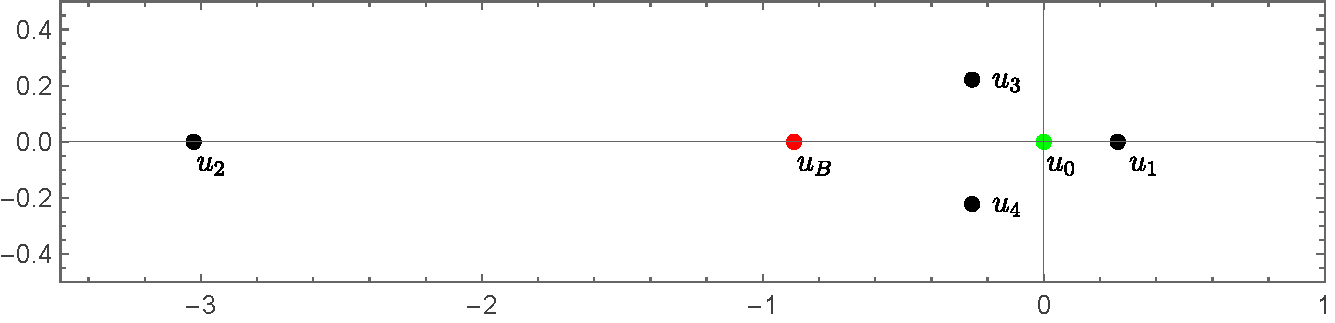
\includegraphics[width=1\textwidth]{UPlaneSingularities_m0}
  \caption{Singularities in the $U$-plane and the branch point.}
  \label{fig:UPlaneSingularities_m0}
\end{figure}

The discriminant of the mirror curve
\begin{equation}
  \mathrm{Disc}(\mathbb{F}_1) = u^8 \qty((16 \lambda ^3-27) u^4-36 \lambda  u^3-8 \lambda ^2 u^2+u+\lambda)
\end{equation}
has five roots, the large volume point (or point of maximal unipotent monodromy, MUM) at $u = 0$ (which is an $I_8$ fiber) and four standard conifold points which we denote $u_1, \dots, u_4$. These are $I_1$ fibers for generic $\lambda$. At $\lambda = 1$, these points are plotted in \cref{fig:UPlaneSingularities_m0}. We generally label the conifold points in this order for $\lambda = 1$ and by continuation to any other $\lambda$ avoiding the singular locus ($\lambda^3 = -27/256$). 

To see that that these are also the singularities of the Picard-Fuchs equations (and additional singularities), we write the third-order PF equations (for periods of the CY3) in this form
\begin{equation}\label{eq:PicardFuchs3}
  \partial_u^3 \varpi(\lambda, u) \ + \ P(\lambda, u) \, \partial_u^2 \varpi(\lambda, u) \ + \ Q(\lambda, u) \, \partial_u \varpi(\lambda, u) = 0
\end{equation}
where $P$ and $Q$ are the following rational functions
\begin{equation}
  P = \frac{24 \lambda ^2+54 \left(16 \lambda ^3-27\right) u^5+4 \lambda  \left(224 \lambda ^3-783\right) u^4-2016 \lambda ^2 u^3+\left(27-320 \lambda ^3\right) u^2+50 \lambda  u}{u (8 \lambda +9 u) \left(\lambda +\left(16 \lambda ^3-27\right) u^4-36 \lambda  u^3-8 \lambda ^2 u^2+u\right)}
\end{equation}
\begin{equation}
  Q = \frac{8 \lambda ^2+54 \left(16 \lambda ^3-27\right) u^5+16 \lambda  \left(64 \lambda ^3-189\right) u^4-1860 \lambda ^2 u^3+\left(9-256 \lambda ^3\right) u^2+16 \lambda  u}{u^2 (8 \lambda +9 u) \left(\lambda +\left(16 \lambda ^3-27\right) u^4-36 \lambda  u^3-8 \lambda ^2 u^2+u\right)}
\end{equation}

From this, it is clear that the only singular points of the third-order PF are $u_0 = 0,\, u_1,\, u_2,\, u_3,\, u_4,\,$ and $u_B = -8\lambda/9$. It is also clear that these are all regular singular points. At $u = 0$, the indicial polynomial is $r^3 = 0$, consistent with it being a MUM point. At $u = u_B = -8\lambda/9$, the indicial polynomial turns out to be $(-3 + r) (-1 + r) r$. At $u = u_i$, $i = 1, 2, 3, 4$, the indicial polynomial is $(-1 + r)^2 r$. At $u = 0$, if we pick a local Frobenius basis
\begin{align}
  \varpi_0 &= 1, \quad \varpi_1 = \log \lambda = 2 \pi \ii m, \\ \varpi_2 &= \log(u) + (\text{analytic}), \\ \varpi_3 &= (\log(u))^2 + \varpi_2 (-2 \log u - \frac{1}{4} \log\lambda) + \frac{(\log \lambda)^2}{8} + (\text{analytic}),
\end{align}
then the large volume periods $T$ and $T_D$ can be written as
\begin{equation}
  T = \frac{\varpi_2}{(2\pi \ii)}, \quad T_D = -4 \frac{\varpi_3}{(2\pi \ii)^2} + \frac{1}{6}.
\end{equation}

\textbf{Method for computing monodromies}

To numerically compute monodromies around the singular points, I define the companion system to \cref{eq:PicardFuchs3},
\begin{equation}
  \partial_u Y(u) = A(u) Y(u)
\end{equation}
where we define the system vector $Y(u)$ and the connection matrix $A(u)$ as,
\begin{equation}
  Y(u) = \begin{pmatrix}
    \varpi(u) \\ \partial_u \varpi(u) \\ \partial_u^2 \varpi(u)
  \end{pmatrix}, \quad A(u) = \begin{pmatrix}
      0 & 1 & 0 \\ 0 & 0 & 1 \\ 0 & -P(u) & -Q(u)
    \end{pmatrix}.
\end{equation}

We define the fundamental matrix $\Phi(u)$ for the fundamental solutions $\varpi_1(u), \varpi_2(u), \varpi_3(u)$ as
\begin{equation}
  \Phi(u) = \begin{pmatrix}
    \varpi_1 & \varpi_2 & \varpi_3 \\ \partial_u \varpi_1 & \partial_u \varpi_2 & \partial_u \varpi_3 \\ \partial_u^2 \varpi_1 & \partial_u^2 \varpi_2 & \partial_u^2 \varpi_3
  \end{pmatrix},
\end{equation}
which also satisfies $\partial_u \Phi(u) = A(u) \Phi(u)$. Thus, to compute monodromies around closed paths $\gamma: [0, 1] \to \mathbb{P}^1/\{u_i\},  t \mapsto u(t)$, we can numerically solve the ODE
\begin{equation}
  \dot{\Psi}(t) = \dot{u}(t) \, A(u(t)) \Psi(t),
\end{equation}
with any initial condition e.g. ($\Psi(0) = I_3$), and then compute the change-of-basis matrix $C$ at the base-point $u_* = u(0)$ which we can take to be inside a small disc around $u_0 = 0$ where we know the period expansions well. The matrix $C$ is given by
\begin{equation}
  C = \begin{pmatrix}
    1 & T(u_*) & T_D(u_*) \\ 0 & \partial_u T(u_*) & \partial_u T_D(u_*) \\ 0 & \partial_u^2 T(u_*) & \partial_u^2 T_D(u_*)
  \end{pmatrix},
\end{equation} 
and the local monodromy around path $\gamma$ is given by
\begin{equation}
  M_\gamma = C^{-1} \Psi(1) C.
\end{equation}

\textbf{Monodromies at $\lambda = 1$}

Using the procedure described above, we find the following monodromies in the $(1, m, T, T_D)$ basis where the second column is deduced by changing $m$ slightly and comparing the first column of the $3 \times 3$ monodromy on $(1, T, T_D)$ computed by numerics \par
\textit{Around $u = 0$:}
\begin{equation}
  M_{LV} = \begin{pmatrix}
    1 & 0 & 0 \\
    1 & 1 & 0 \\
    4 & 8 & 1
  \end{pmatrix} \ \to \ \begin{pmatrix}
    1 & 0 & 0 & 0 \\
    0 & 1 & 0 & 0 \\
    1 & 0 & 1 & 0 \\
    4 & 1 & 8 & 1
  \end{pmatrix}
\end{equation}

\textit{Around $u = u_B = -8\lambda/9$:}
\begin{equation}
  M_B = I_3 \ \to \ I_4
\end{equation}




% \subsubsection{Systematic checklist (``algorithm'')}
% To ensure no special cases are missed, proceed as follows.
% \begin{enumerate}
% \item \textbf{Compute and factor the discriminant} $\Disc_u(P(u;J,\ell))$ as a polynomial in $J$:
% its roots are the branch values; their multiplicities encode how many sheets collide.
% \item \textbf{Compute and factor} $\mathrm{num}\!\left(\frac{dJ}{du}\right)$:
% the critical factors (here $\ur$, $9u+8$, $Q$, $S$) determine preimages and ramification indices.
% \item \textbf{Find special parameters} where the Hurwitz data changes:
% \[
% \Res_u(N,u^8E)=0,\quad
% \Disc_u(Q)=0,\quad
% \Disc_u(S)=0,
% \]
% and solve collision equations among branch values, e.g.
% \[
% J_B(\ell)\in\{0,1728,\infty\},\qquad
% J_B(\ell)=J(\infty;\ell),\qquad
% J(\infty;\ell)\in\{0,1728,\infty\}.
% \]
% \end{enumerate}
% These loci stratify the $\ell$-line into chambers on which the covering $\phi_\ell$ has
% constant degree and constant ramification profile.

\subsection{Branch point analysis}
\subsubsection{Period expansion near \texorpdfstring{$\ur = -\frac{8}{9}$}{ur = -8/9}}
The third order Picard-Fuchs equation for the periods of local $\mathbb{F}_1$ can be written as $\mathcal{D}_3 \varpi(\ell, \ur) = 0$, with
\begin{equation}
  \mathcal{D}_3 = \partial_\ur^3 + P(\ell, \ur) \partial_\ur^2 + Q(\ell, \ur) \partial_\ur,
\end{equation}
\begin{equation}
  \begin{aligned}
    P(\ell, \ur) &= \frac{54 \ell (16 \ell-27) \ur^5+4 \ell (224 \ell-783) \ur^4-2016 \ell \ur^3+(27-320 \ell) \ur^2+50 \ur+24}{\delta(\ell, \ur)}, \\
    Q(\ell, \ur) &= \frac{54 \ell (16 \ell-27) \ur^5+16 \ell (64 \ell-189) \ur^4-1860 \ell \ur^3+(9-256 \ell) \ur^2+16 \ur+8}{\ur \, \delta(\ell, \ur)}, \\
    \delta(\ell, \ur) &= \ur (9 \ur+8) \left(\ell (16 \ell-27) \ur^4-36 \ell \ur^3-8 \ell \ur^2+\ur+1\right)
  \end{aligned}
\end{equation}

The point $\ur = -\tfrac89$ is a regular singular point with local exponents $(0, 1, 3)$ for generic values of $\ell$ and $(0, \tfrac56, \tfrac76)$ at $\ell = -\frac{27}{256}$. The solutions can be written in terms of $\ur = -8/9 + z$ in the canonical Frobenius basis as follows
\begin{equation}
  \begin{aligned}
    \varpi_0 &= 1, \\
    \varpi_1 &= z+\frac{9 (512 \ell+27) z^2}{4096 \ell+432}-\frac{729 \left(67108864 \ell^3-4423680 \ell^2-559872 \ell-45927\right) z^4}{1024 (256 \ell+27)^3}+\mathcal{O}(z^5), \\
    \varpi_2 &= z^3+\frac{27 (1024 \ell-99) z^4}{8192 \ell+864}+\frac{243 \left(1310720 \ell^2-211968 \ell+36207\right) z^5}{640 (256 \ell+27)^2}\\
    &\qquad +\frac{729 \left(671088640 \ell^3-130940928 \ell^2+36951552 \ell-6187023\right) z^6}{2048 (256 \ell+27)^3} +\mathcal{O}(z^7)
  \end{aligned}
\end{equation}

The periods are $\ell$-dependent combinations of $\varpi_i$,
\begin{equation}
  \varpi(\ell, \ur) = \alpha_0(\ell) \varpi_0 + \alpha_1(\ell) \varpi_1 + \alpha_2(\ell) \varpi_2
\end{equation}

We can fix the $\ell$ dependence by using the original Picard-Fuchs equations which read $\mathcal{D}_i \varpi(\ell, \ur) = 0$
\begin{equation}\label{eq:PicardFuchsD1D2}
  \begin{gathered}
    \mathcal{D}_1 = -\ur^4 \partial_\ur^2-2 \ur^3 \partial_\ur-\ur \partial_\ur \partial_\ell+3 \partial_\ell+3 \ell \partial_\ell^2, \\
    \mathcal{D}_2 = (\ur+1) \ur \left(\ur \partial_\ur^2+ \partial_\ur\right) +\ell \left(4 \partial_\ell-\ur (3 \ur+4) \partial_\ell \partial_\ur +4 \ell \partial_\ell^2\right).
  \end{gathered}
\end{equation}
The result is a set of ordinary differential equations for the coefficients $\alpha_i(\ell)$,
\begin{gather}
  \ell (256 \ell+27)^2 \alpha_1''(\ell)+(512 \ell+27) (256 \ell+27) \alpha_1'(\ell)+(16384 \ell+1920) \alpha_1(\ell) = 0, \label{eq:pf-branch-point-1}\\
  \ell \alpha_0''(\ell)+\alpha_0'(\ell)+\frac{8}{27}\alpha_1'(\ell)+\frac{512}{81(256 \ell+27)}\alpha_1(\ell)=0, \label{eq:pf-branch-point-2}\\
  \alpha_2(\ell) = \frac{81 \left(\left(65536 \ell^2-3456 \ell+243\right) \alpha_1(\ell)-\left(27648 \ell^2+2916 \ell\right) \alpha_1'(\ell)\right)}{64 (256 \ell+27)^2}
\end{gather}

The first equation can be solved in terms of hypergeometric functions. Let $z = -\tfrac{256}{27} \ell$, we make the gauge transformation,
\begin{equation}
  \alpha_1(z) = (1 - z)^{-\tfrac16} u(z),
\end{equation}
This transforms \cref{eq:pf-branch-point-1} into
\begin{equation}
  z (z-1) \, u''(z) + \qty(\frac{5 z}{3}-1) \, u'(z) + \frac19 u(z) = 0
\end{equation}
which can be recognized as the Gauss hypergeometric equation with $(a, b, c) = \qty(\tfrac13, \tfrac13, 1)$. Thus the solutions are
\begin{equation}
  \begin{aligned}
    u_1(z) &= \hypF{\tfrac13}{\tfrac13}{1}{z}, \\
    u_2(z) &= -\frac{2\pi}{\sqrt{3}} \, \hypF{\tfrac13}{\tfrac13}{1}{z} - \Gamma\!\left(\tfrac23\right)^2 G^{2,0}_{2,2}\!\left(
      z \,\Bigg|\,
      \begin{matrix}
      \tfrac23,\,\tfrac23\\
      0,\,0
      \end{matrix}
      \right) \\
    &=\hypF{\tfrac13}{\tfrac13}{1}{z} \log z + \sum_{k=0}^{\infty}\frac{\left(\frac{1}{3}\right)_{k}^{2}}{(k!)^{2}}\,z^{k}
      \left[\,2\,\psi\!\left(k+\frac{1}{3}\right)-2\,\psi(k+1)\right].
  \end{aligned}
\end{equation}
This gives us a solution for $\alpha_1$ but leaves the more important contribution $\alpha_0$ still unknown. $\alpha_0$ seems to satisfy a first-order ODE with a source term given by combinations of $u_1$ and $u_2$ above which would not be solvable analytically.

\paragraph{Strategy 1}
It is interesting to analyze the differential equation satisfied by the source term for \cref{eq:pf-branch-point-2},
\begin{equation}
  \mathrm{src}(\ell) = -\frac{8}{81} \left(3 \alpha _1'(\ell )+\frac{64 \alpha _1(\ell )}{256 \ell +27}\right)
\end{equation}
By taking the first and second derivatives of $\mathrm{src}$, and using the equation for $\alpha_0$ \cref{eq:pf-branch-point-1}, we find the following equation for $\mathrm{src}$,
\begin{equation}
  \begin{aligned}
    \mathrm{src}''(\ell) &+ \frac{2 \left(819200 \ell ^2+142560 \ell +5103\right)}{\ell  \left(409600 \ell ^2+91584 \ell +5103\right)} \mathrm{src}'(\ell) \\
    &\quad + \frac{3840 \left(61440 \ell ^2+14240 \ell +783\right)}{\ell  (256 \ell +27)^2 (1600 \ell +189)} \mathrm{src}(\ell) = 0
  \end{aligned}
\end{equation}
or, in terms of $z = -\tfrac{256}{27}\ell$,
\begin{equation}
  \mathrm{src}''(z) + \frac{100 z^2-165 z+56}{25 z^3-53 z^2+28 z} \mathrm{src}'(z) + \frac{5 \left(405 z^2-890 z+464\right)}{36 (z-1)^2 z (25 z-28)} \mathrm{src}(z) = 0
\end{equation}
The Fuchsian data is as follows (note that in all of the rest of this section, by point, I mean a regular singular point),
\begin{equation}
\begin{tabular}{c|c}
point & exponents \\
\hline
$z=0$      & $(0, -1)$ \\
$z=1$      & $(-\tfrac76, -\tfrac56)$ \\
$z=\tfrac{28}{25}$ & $(0, 2)$ \\
$z=\infty$ & $(\tfrac32, \tfrac32)$ \\
\end{tabular}
\end{equation}
which motivates the following gauge transformation
\begin{equation}
  \mathrm{src}(z) = (z-1)^{-\tfrac76} \, u(z)
\end{equation}
which leads to the ODE
\begin{equation}
  9 z \left(25 z^2-53 z+28\right) u''(z)+\left(375 z^2-897 z+504\right) u'(z)+(25 z+8) u(z) = 0
\end{equation}
with Fuchsian data
\begin{equation}
\begin{tabular}{c|c}
point & exponents \\
\hline
$z=0$      & $(0, -1)$ \\
$z=1$      & $(0, \tfrac13)$ \\
$z=\tfrac{28}{25}$ & $(0, 2)$ \\
$z=\infty$ & $(\tfrac13, \tfrac13)$ \\
\end{tabular}
\end{equation}
which can be recognized as the Fuchsian data of the Heun equation,
\begin{equation}
  w''(z) + \left[ \frac{\gamma}{z} + \frac{\delta}{z-1} + \frac{\epsilon}{z-a} \right] w'(z) + \frac{\alpha \beta z - q}{z(z-1)(z-a)} w(z) = 0
\end{equation}
with $a = \frac{28}{25}$, $\gamma=2$, $\delta = \tfrac23$, $\epsilon = -1$, $q = -\frac{8}{225}$, $\alpha = \beta = \tfrac13$. Thus the most general solution is
\begin{equation}
  u(z) = c_2 \HeunG\!\left(\frac{28}{25},-\frac{8}{225};\frac{1}{3},\frac{1}{3}, 2,\frac{2}{3};\,z\right) \, + \, \frac{c_3}{z} \HeunG\!\left(\frac{28}{25},\frac{49}{225};-\frac{2}{3},-\frac{2}{3}, 0,\frac{2}{3};\,z\right)
\end{equation}

\paragraph{Strategy 2}
Another strategy to solve for $\alpha_0$ is to uncouple $\alpha_1$ from it and obtain a single equation for $\alpha_0$. Performing this, we find the following fourth order linear ODE
\begin{equation}
\begin{aligned}
&3840\bigl(61440\,\ell^{2}+14240\,\ell+783\bigr)\,\alpha_{0}'(\ell)\\
&\quad+4\bigl(268697600\,\ell^{3}+72284160\,\ell^{2}+5907168\,\ell+137781\bigr)\,\alpha_{0}''(\ell)\\
&\quad+\ell\,(256\ell+27)\bigl(2867200\,\ell^{2}+559872\,\ell+25515\bigr)\,\alpha_{0}^{(3)}(\ell)\\
&\quad+\ell^{2}\,(256\ell+27)\bigl(409600\,\ell^{2}+91584\,\ell+5103\bigr)\,\alpha_{0}^{(4)}(\ell) = 0
\end{aligned}
\end{equation}
Writing $\ell = -\tfrac{27}{256}z$, the equation reduces to
\begin{equation}
\begin{aligned}
&5\bigl(405 z^{2}-890 z+464\bigr)\,\alpha_{0}'(z)
+\bigl(9225 z^{3}-23530 z^{2}+18232 z-4032\bigr)\,\alpha_{0}''(z)\\
&\quad+36(z-1)z\,\bigl(175 z^{2}-324 z+140\bigr)\,\alpha_{0}^{(3)}(z)\\
&\quad+36(z-1)z^{2}\,\bigl(25 z^{2}-53 z+28\bigr)\,\alpha_{0}^{(4)}(z)
=0.
\end{aligned}
\end{equation}

We know that the homogenous solutions to the original equation \cref{eq:pf-branch-point-2}, $1$ and $\log \ell$ must still be solutions to this fourth order equation and indeed they are. One may ask if this lets us factorize this equation into a second order ODE times the annihiator of $1$ and $\log$. To that end, let us write the equation in terms of $\theta = z \partial_z$. We find that the fourth order operator $\mathcal{D}_4$ can be factored as follows
\begin{equation}
  \begin{aligned}
    \mathcal{D}_4 &= \mathcal{D}_2 \theta^2 \\
    \mathcal{D}_2 &= \theta^2 + \frac{25 z^2-6 z-28}{25 z^2-53 z+28} \theta + \frac{z \left(225 z^2-526 z+196\right)}{36 (z-1)^2 (25 z-28)}
  \end{aligned}
\end{equation}
$\mathcal{D}_2$ has the following Fuchsian data
\begin{equation}
\begin{tabular}{c|c}
point & exponents \\
\hline
$z=0$      & $(0, 1)$ \\
$z=1$      & $(-\tfrac76, -\tfrac56)$ \\
$z=\tfrac{28}{25}$ & $(0, 2)$ \\
$z=\infty$ & $(\tfrac12, \tfrac12)$ \\
\end{tabular}
\end{equation}
After the guage transformation, $f(z) \to (z-1)^{-\tfrac76} f(z)$, we find the following equation and data
\begin{equation}
  \begin{aligned}
  &\mathcal{D}_2'f(z) = f''(z) + \left( \frac{2}{3 (z-1)}-\frac{1}{z-\frac{28}{25}} \right) f'(z) + \frac{\frac{4 z}{9}-\frac{49}{225}}{z(z-1)(z-\frac{28}{25})} f(z) = 0 \\
&\begin{tabular}{c|c}
point & exponents \\
\hline
$z=0$      & $(0, 1)$ \\
$z=1$      & $(0, \tfrac13)$ \\
$z=\tfrac{28}{25}$ & $(0, 2)$ \\
$z=\infty$ & $(-\tfrac23, -\tfrac23)$ \\
\end{tabular}
\end{aligned}
\end{equation}
which is another Heun equation. The solution is given by
\begin{equation}
  f(z) = c_2' \HeunG\!\left(\frac{28}{25},\frac{49}{225};-\frac{2}{3},-\frac{2}{3}, 0,\frac{2}{3};\,z\right) + c_3' \, z \HeunG\!\left(\frac{28}{25},-\frac{8}{225};\frac{1}{3},\frac{1}{3}, 2,\frac{2}{3};\,z\right)
\end{equation}
which is the same as in strategy 1 upto a basis change and a gauge transformation.

We are thus led to solving the equation
\begin{equation}
  \theta^2 \alpha_0(z) = \mathcal{D}_2^{-1}(0) = (z-1)^{-\tfrac76} f(z)
\end{equation}

Formally, the solution is given by
\begin{equation}
  \alpha_0(z) = C_0 + C_1 \log z + \int^z \frac{\dd{\xi}}{\xi} \int^{\xi} \dd{\eta} (\eta-1)^{-\tfrac76} \frac{f(\eta)}{\eta}
\end{equation}



\section{4d Seiberg--Witten with \texorpdfstring{$N_f = 1$}{Nf=1} matter hypermultiplets}

\subsection{Mutation class of a three-node quiver}

Consider the three-node quiver
\[
2 \xrightarrow{2} 1,\qquad 1\to 3,\qquad 3\to 2 .
\]
Equivalently, using the skew-symmetric exchange matrix convention
\[
B_{ij}=\#(i\to j)-\#(j\to i),
\]
we have
\[
B_0=
\begin{pmatrix}
0&-2&1\\
2&0&-1\\
-1&1&0
\end{pmatrix}.
\]

Mutation at a node \(k\) is defined by
\[
b'_{ij}=
\begin{cases}
-b_{ij}, & i=k\ \text{or}\ j=k,\\[4pt]
b_{ij}+[b_{ik}]_+[b_{kj}]_+
      -[-b_{ik}]_+[-b_{kj}]_+, & i,j\neq k,
\end{cases}
\]
where \([x]_+=\max(x,0)\). In quiver language, this means: for every path
\(i\to k\to j\), add an arrow \(i\to j\), then reverse all arrows incident
on \(k\), and finally cancel oriented 2-cycles.

For example, mutating \(B_0\) at node \(3\), the path
\[
1\to 3\to 2
\]
adds one arrow \(1\to 2\), which cancels one of the two arrows \(2\to 1\).
After reversing the arrows adjacent to \(3\), one obtains
\[
2\to1,\qquad 3\to1,\qquad 2\to3.
\]

Iterating mutations at the three nodes gives a finite labelled mutation
class with \(12\) quivers:
\[
\begin{array}{c|l}
Q_0 & 2\xrightarrow{2}1,\ 1\to3,\ 3\to2\\
Q_1 & 1\xrightarrow{2}2,\ 3\to1,\ 2\to3\\
Q_2 & 2\to1,\ 3\to1,\ 2\to3\\
Q_3 & 1\to2,\ 1\to3,\ 3\to2\\
Q_4 & 1\to2,\ 1\to3,\ 2\to3\\
Q_5 & 1\to2,\ 3\to1,\ 3\to2\\
Q_6 & 2\to1,\ 3\to1,\ 3\to2\\
Q_7 & 2\to1,\ 1\to3,\ 2\to3\\
Q_8 & 2\to1,\ 1\xrightarrow{2}3,\ 3\to2\\
Q_9 & 2\to1,\ 1\to3,\ 3\xrightarrow{2}2\\
Q_{10} & 1\to2,\ 3\xrightarrow{2}1,\ 2\to3\\
Q_{11} & 1\to2,\ 3\to1,\ 2\xrightarrow{2}3
\end{array}
\]

Thus the labelled mutation class has size
\[
|\operatorname{Mut}(Q_0)|=12.
\]
Up to relabelling of the nodes, there are only two underlying shapes:
a cyclic triangle with arrow multiplicities \((2,1,1)\), and an acyclic
triangle with multiplicities \((1,1,1)\). In particular, the quiver is
mutation-equivalent to an acyclic orientation of the affine
\(\widetilde A_2\) triangle.



\appendix

\subsection{Mutation class of the three-node quiver for \texorpdfstring{\(SU(2)\)}{SU(2)}, \texorpdfstring{\(N_f=1\)}{Nf=1}}

The strong-coupling quiver of pure \(SU(2)\) Seiberg--Witten theory is the
two-node, two-arrow Kronecker quiver. A convenient basis of charges for its two
nodes is
\[
\gamma_a=(n_e,n_m)=(0,1),\qquad
\gamma_b=(n_e,n_m)=(-1,1).
\]
If one adds a very massive quark and then later takes the decoupling limit
\(m\to \infty\), the resulting theory must reduce back to the pure SW theory.
Thus the \(N_f=1\) quiver should be obtained by adjoining one extra node to the
two-node quiver. A natural choice for the third charge is
\[
\gamma_c=(-2,1).
\]

With the Dirac--Schwinger--Zwanziger pairing
\[
\langle (n_e,n_m),(n_e',n_m')\rangle
= n_e n_m' - n_m n_e',
\]
one finds
\[
\langle \gamma_a,\gamma_b\rangle =1,\qquad
\langle \gamma_b,\gamma_c\rangle =1,\qquad
\langle \gamma_a,\gamma_c\rangle =2.
\]
Hence, up to the usual convention for arrow orientation and relabelling of the
nodes, the seed quiver is the cyclic three-node quiver with arrow
multiplicities \((2,1,1)\). We take as seed
\[
Q_0:\qquad 2\xrightarrow{2}1,\qquad 1\to3,\qquad 3\to2.
\]
Equivalently, in terms of the exchange matrix
\[
B_{ij}=\#(i\to j)-\#(j\to i),
\]
the seed is
\[
B_0=
\begin{pmatrix}
0&-2&1\\
2&0&-1\\
-1&1&0
\end{pmatrix}.
\]

Mutation at node \(k\) is defined by
\[
b'_{ij}=
\begin{cases}
-b_{ij}, & i=k\ \text{or}\ j=k,\\[4pt]
b_{ij}+[b_{ik}]_+[b_{kj}]_+
      -[-b_{ik}]_+[-b_{kj}]_+, & i,j\neq k,
\end{cases}
\qquad [x]_+=\max(x,0).
\]
In quiver language: for every path \(i\to k\to j\), add an arrow \(i\to j\);
then reverse all arrows incident on \(k\); finally cancel all oriented
2-cycles.

\paragraph{Remark on charges.}
The mutation class below is the class of \emph{unlabelled quivers}. If one also
wants the \((n_e,n_m)\)-charges carried by the nodes, one must choose either a
left- or a right-mutation convention for the charge basis. For example, under a
right mutation at node \(k\),
\[
\gamma_k'=-\gamma_k,\qquad
\gamma_i'=\gamma_i+[B_{ik}]_+\,\gamma_k,\qquad i\neq k,
\]
while under a left mutation one uses
\[
\gamma_k'=-\gamma_k,\qquad
\gamma_i'=\gamma_i+[B_{ki}]_+\,\gamma_k,\qquad i\neq k.
\]
Thus every quiver in the mutation class comes with a corresponding mutated
charge basis \((\gamma_1',\gamma_2',\gamma_3')\), obtained recursively from the
seed basis. For the purposes of the mutation \emph{class} itself, however, the
unlabelled quivers are enough.

\paragraph{Example.}
Starting from \(Q_0\), mutation at node \(3\) gives
\[
Q_2:\qquad 2\to1,\qquad 3\to1,\qquad 2\to3.
\]
Indeed, the path \(1\to3\to2\) creates one arrow \(1\to2\), which cancels one
of the two arrows \(2\to1\); then the arrows adjacent to node \(3\) are
reversed.

\paragraph{The full labelled mutation class.}
Iterating mutations at nodes \(1,2,3\) produces a finite class of \(12\)
labelled quivers.

%------------------------------------------------------------
% TikZ setup
%------------------------------------------------------------
\begin{center}
\small

\begin{minipage}{0.24\textwidth}\centering
\(Q_0\)

\begin{tikzpicture}[baseline=(current bounding box.center),scale=1]
\qvertices
\draw[qarr] (2) -- node[midway,left,fill=white,inner sep=1pt] {$2$} (1);
\draw[qarr] (1) -- (3);
\draw[qarr] (3) -- (2);
\end{tikzpicture}
\end{minipage}
\begin{minipage}{0.24\textwidth}\centering
\(Q_1\)

\begin{tikzpicture}[baseline=(current bounding box.center),scale=1]
\qvertices
\draw[qarr] (1) -- node[midway,left,fill=white,inner sep=1pt] {$2$} (2);
\draw[qarr] (3) -- (1);
\draw[qarr] (2) -- (3);
\end{tikzpicture}
\end{minipage}
\begin{minipage}{0.24\textwidth}\centering
\(Q_2\)

\begin{tikzpicture}[baseline=(current bounding box.center),scale=1]
\qvertices
\draw[qarr] (2) -- (1);
\draw[qarr] (3) -- (1);
\draw[qarr] (2) -- (3);
\end{tikzpicture}
\end{minipage}
\begin{minipage}{0.24\textwidth}\centering
\(Q_3\)

\begin{tikzpicture}[baseline=(current bounding box.center),scale=1]
\qvertices
\draw[qarr] (1) -- (2);
\draw[qarr] (1) -- (3);
\draw[qarr] (3) -- (2);
\end{tikzpicture}
\end{minipage}

\medskip

\begin{minipage}{0.24\textwidth}\centering
\(Q_4\)

\begin{tikzpicture}[baseline=(current bounding box.center),scale=1]
\qvertices
\draw[qarr] (1) -- (2);
\draw[qarr] (1) -- (3);
\draw[qarr] (2) -- (3);
\end{tikzpicture}
\end{minipage}
\begin{minipage}{0.24\textwidth}\centering
\(Q_5\)

\begin{tikzpicture}[baseline=(current bounding box.center),scale=1]
\qvertices
\draw[qarr] (1) -- (2);
\draw[qarr] (3) -- (1);
\draw[qarr] (3) -- (2);
\end{tikzpicture}
\end{minipage}
\begin{minipage}{0.24\textwidth}\centering
\(Q_6\)

\begin{tikzpicture}[baseline=(current bounding box.center),scale=1]
\qvertices
\draw[qarr] (2) -- (1);
\draw[qarr] (3) -- (1);
\draw[qarr] (3) -- (2);
\end{tikzpicture}
\end{minipage}
\begin{minipage}{0.24\textwidth}\centering
\(Q_7\)

\begin{tikzpicture}[baseline=(current bounding box.center),scale=1]
\qvertices
\draw[qarr] (2) -- (1);
\draw[qarr] (1) -- (3);
\draw[qarr] (2) -- (3);
\end{tikzpicture}
\end{minipage}

\medskip

\begin{minipage}{0.24\textwidth}\centering
\(Q_8\)

\begin{tikzpicture}[baseline=(current bounding box.center),scale=1]
\qvertices
\draw[qarr] (2) -- (1);
\draw[qarr] (1) -- node[midway,right,fill=white,inner sep=1pt] {$2$} (3);
\draw[qarr] (3) -- (2);
\end{tikzpicture}
\end{minipage}
\begin{minipage}{0.24\textwidth}\centering
\(Q_9\)

\begin{tikzpicture}[baseline=(current bounding box.center),scale=1]
\qvertices
\draw[qarr] (2) -- (1);
\draw[qarr] (1) -- (3);
\draw[qarr] (3) -- node[midway,below,fill=white,inner sep=1pt] {$2$} (2);
\end{tikzpicture}
\end{minipage}
\begin{minipage}{0.24\textwidth}\centering
\(Q_{10}\)

\begin{tikzpicture}[baseline=(current bounding box.center),scale=1]
\qvertices
\draw[qarr] (1) -- (2);
\draw[qarr] (3) -- node[midway,right,fill=white,inner sep=1pt] {$2$} (1);
\draw[qarr] (2) -- (3);
\end{tikzpicture}
\end{minipage}
\begin{minipage}{0.24\textwidth}\centering
\(Q_{11}\)

\begin{tikzpicture}[baseline=(current bounding box.center),scale=1]
\qvertices
\draw[qarr] (1) -- (2);
\draw[qarr] (3) -- (1);
\draw[qarr] (2) -- node[midway,below,fill=white,inner sep=1pt] {$2$} (3);
\end{tikzpicture}
\end{minipage}

\end{center}

Therefore the labelled mutation class has size
\[
|\mathrm{Mut}(Q_0)|=12.
\]
Up to relabelling, there are only two underlying shapes:
\begin{itemize}
\item the cyclic quiver with multiplicities \((2,1,1)\);
\item the acyclic quiver with multiplicities \((1,1,1)\).
\end{itemize}
Thus the seed quiver for \(SU(2)\), \(N_f=1\) is mutation-equivalent to an
acyclic orientation of the affine \(\widetilde A_2\) triangle.

\paragraph{Comment on the charges across the mutation class.}
The seed basis may be taken to be
\[
(\gamma_1,\gamma_2,\gamma_3)\sim \bigl((0,1),\,(-1,1),\,(-2,1)\bigr),
\]
up to relabelling and overall sign conventions. Each quiver \(Q_i\) in the
mutation class carries a basis of charges obtained by successive left or right
mutations from this seed basis. The underlying quiver only remembers the DSZ
pairings among the basis elements, whereas the actual node charges depend on the
chosen mutation convention. Hence, when needed, it is best to keep the quiver
diagram and the mutated charge basis as separate pieces of data.



\section{Degenerations of the map \texorpdfstring{$\ur \mapsto J$}{ur -> J}}
\label{sec:degenerations-J-ur}

Fix the parameter $\ell \in \C$ and consider the rational map
\begin{equation}
\label{eq:Jmap}
J(\ur;\ell)
=
\frac{N(\ur;\ell)^3}{\ell^3\,\ur^8\,E(\ur;\ell)},
\end{equation}
where
\begin{align}
\label{eq:Nu}
N(\ur;\ell)
&:=1+16\ell^2 \ur^4-8\ell \ur^2(1+3\ur),
\\
\label{eq:Eu}
E(\ur;\ell)
&:=1+\ur-8\ell \ur^2-36\ell \ur^3+\ell(-27+16\ell)\ur^4.
\end{align}
For generic $\ell$, the map \eqref{eq:Jmap} defines a degree-$12$ cover
\(
\phi_\ell:\PP^1_\ur \to \PP^1_J
\)
(i.e.\ generically $12$ preimages for a given $J$).

\subsection{Branch values via the discriminant method}
For fixed $\ell$, branch values $J_\ast$ are characterized by the condition that the fiber
\(
\phi_\ell^{-1}(J_\ast)
\)
has multiplicities, i.e.\ that the equation $J(\ur;\ell)=J$ has a multiple root in $\ur$.
Equivalently, define the polynomial in $\ur$
\begin{equation}
\label{eq:Pu}
P(\ur;J,\ell):=N(\ur;\ell)^3 - J\,\ell^3 \ur^8 E(\ur;\ell).
\end{equation}
Then $J$ is a branch value of $\phi_\ell$ if and only if
\begin{equation}
\label{eq:disc-condition}
\Disc_\ur\bigl(P(\ur;J,\ell)\bigr)=0.
\end{equation}
After factoring, one finds that (up to an overall nonzero constant)
\begin{equation}
\label{eq:disc-factor}
\Disc_\ur\bigl(P(\ur;J,\ell)\bigr)
=
J^{8}(J-1728)^{6}\bigl(J-J_B(\ell)\bigr)\cdot \ell^{44}(256\ell+27)^3.
\end{equation}
Hence for generic $\ell\neq 0,-\tfrac{27}{256}$ the branch values on the $J$-sphere are
\begin{equation}
\label{eq:branchvalues-generic}
J \in \{0,\;1728,\;J_B(\ell),\;\infty\},
\qquad
J_B(\ell)=\frac{(256\ell+27)(256\ell+243)^3}{2^{24}\,\ell^3}.
\end{equation}

\subsection{Critical points and generic ramification profile}
Critical points in the $\ur$-sphere are the zeros of $\frac{dJ}{d\ur}$.
Writing $\frac{dJ}{d\ur}=\frac{\mathrm{num}}{\mathrm{den}}$, the numerator factorizes as
\begin{equation}
\label{eq:dJdu-factor}
\mathrm{num}\!\left(\frac{dJ}{d\ur}\right)
=
\ell^{3}\ur^{7}(9\ur+8)\,Q(\ur;\ell)^2\,S(\ur;\ell),
\end{equation}
where
\begin{align}
\label{eq:Q}
Q(\ur;\ell)&:=16\ell^2\ur^4-24\ell \ur^3-8\ell \ur^2+1,
\\
\label{eq:S}
S(\ur;\ell)&:=64\ell^3\ur^6-216\ell^2\ur^6-144\ell^2\ur^5-48\ell^2\ur^4+36\ell \ur^3+12\ell \ur^2-1.
\end{align}
For generic $\ell$, the ramification data over the branch values in
\eqref{eq:branchvalues-generic} is:
\begin{itemize}
\item Over $J=\infty$: $\ur=0$ is an order-$8$ pole, hence ramification index $e=8$
(contribution $e-1=7$). The remaining poles are the simple roots of $E(\ur;\ell)$.
\item Over $J=0$: $N(\ur;\ell)=0$ is equivalent to $Q(\ur;\ell)=0$ (since $N$ is quartic),
and the square $Q^2$ in \eqref{eq:dJdu-factor} implies that each root of $Q$ is
ramified with $e=3$. Thus the fiber over $0$ has cycle type
\[
3+3+3+3.
\]
\item Over $J=1728$: the six roots of $S(\ur;\ell)$ map to $1728$ and are simple critical
points, giving cycle type
\[
2+2+2+2+2+2.
\]
\item Over $J=J_B(\ell)$: the factor $(9\ur+8)$ shows that $\ur=-\frac{8}{9}$ is a simple
critical point, hence contributes one transposition; the remaining ten points are
unramified. Cycle type:
\[
2+1+\cdots+1 \quad (\text{ten $1$'s}).
\]
\end{itemize}

\subsection{What it means for the map to ``degenerate''}
There are two distinct sources of degeneration.

\paragraph{(I) Special branch values for fixed $\ell$.}
For fixed $\ell$, the fiber over $J$ ceases to consist of $12$ distinct points precisely
when \eqref{eq:disc-condition} holds. The branch values are therefore
\eqref{eq:branchvalues-generic}, and multiplicities are encoded in the factorization of
the discriminant \eqref{eq:disc-factor}.

\paragraph{(II) Special parameters $\ell$ where the cover changes type.}
As $\ell$ varies, the Hurwitz data (cycle types, collisions of branch values, degree)
can change at parameter values where:
\begin{enumerate}
\item \textbf{Cancellation (degree drop):} numerator and denominator share a common factor,
i.e.\ $\gcd\bigl(N(\ur;\ell)^3,\ell^3\ur^8E(\ur;\ell)\bigr)\neq 1$.
Equivalently, $\Res_\ur\bigl(N(\ur;\ell),u^8E(\ur;\ell)\bigr)=0$.
\item \textbf{Critical points collide:} $\Disc_\ur(Q(\ur;\ell))=0$ or $\Disc_\ur(S(\ur;\ell))=0$.
\item \textbf{Branch values collide:} $J_B(\ell)$ hits $\{0,1728,\infty\}$ or merges with
the value $J(\infty)$ (see below).
\end{enumerate}

\subsection{Distinguished special values of \texorpdfstring{$\ell$}{el} (explicit list)}
The following parameter values are singled out by the above mechanisms:
\begin{itemize}
\item \textbf{Ill-defined family point:} $\ell=0$ (the formula \eqref{eq:Jmap} has $\ell^3$
in the denominator).
\item \textbf{True cancellation / degree drop:}
\begin{equation}
\label{eq:ell-cancel}
\ell=-\frac{27}{256}.
\end{equation}
At this value numerator and denominator share a nontrivial common factor in $\ur$, so after
cancellation the degree drops below $12$.
\item \textbf{Collision in the $J=0$ fiber (ramification increases):}
\begin{equation}
\label{eq:ell-Qdisc}
\ell=-\frac{243}{256}.
\end{equation}
Here $Q(\ur;\ell)$ acquires a repeated root at $\ur=-\frac{8}{9}$, changing the cycle type
over $J=0$.
\item \textbf{Collision in the $J=1728$ fiber and branch-value collision $J_B(\ell)=1728$:}
\begin{equation}
\label{eq:ell-Sdisc}
\ell=\frac{243}{256}\pm\frac{81\sqrt{3}}{128},
\end{equation}
equivalently the roots of
\(
65536\ell^2-124416\ell-19683=0.
\)
These are characterized by $\Disc_\ur(S(\ur;\ell))=0$ and simultaneously $J_B(\ell)=1728$.
\end{itemize}

\subsection{Behavior at \texorpdfstring{$u=\infty$}{u = infinity} and additional special values}
The value of the map at infinity is obtained from the leading terms:
\begin{equation}
\label{eq:J-infty}
J(\infty;\ell)=\lim_{u\to\infty}J(u;\ell)=\frac{4096\,\ell^2}{16\ell-27},
\qquad (\ell\neq 27/16).
\end{equation}
This exhibits further distinguished parameters:
\begin{itemize}
\item $\ell=\frac{27}{16}$: the leading term of $E(\ur;\ell)$ vanishes, so $J(\infty;\ell)=\infty$
(i.e.\ a pole effectively moves to $\ur=\infty$).
\item $\ell=\frac{27}{8}$: one has $J(\infty;\ell)=1728$; in addition $\ur=\infty$ becomes
ramified (the local expansion starts at order $(1/\ur)^2$), producing extra branching over
$J=1728$.
\end{itemize}


\section{Domain, range, and branching structure of the map \texorpdfstring{$\ell(b)$}{el(b)}}
\label{sec:domain-range-branching-ell-of-b}

Consider the rational map of Riemann spheres
\begin{equation}
  \ell:\PP^1_b \longrightarrow \PP^1_\ell,
  \qquad
  \ell(b) \;=\; -\frac{b\,(1+b+b^2)^3}{(1+b)^8}\,.
\end{equation}
Since $\ell$ is a non-constant holomorphic map $\PP^1\to\PP^1$, it is surjective onto $\PP^1_\ell$; the interesting features are its divisor, critical points, and branch values.

\subsection{Divisor data: zeros and poles}
The only pole occurs at $b=-1$, with order $8$:
\begin{equation}
  \ell(b) \sim -\frac{(-1)\,(1-1+1)^3}{(b+1)^8}
  \quad\text{as } b\to -1,
  \qquad\Rightarrow\qquad
  \ord_{b=-1}(\ell)=-8,\ \ \ell(-1)=\infty.
\end{equation}
The numerator vanishes at $b=0$ (simple) and at the primitive cube roots of unity $b=\om,\om^2$ (each with multiplicity $3$). In addition, as $b\to\infty$,
\begin{equation}
  \ell(b)= -\frac{b(b^2)^3}{b^8}\,\bigl(1+O(1/b)\bigr)
  = -\frac{1}{b}\,\bigl(1+O(1/b)\bigr),
\end{equation}
so $\ell(\infty)=0$ and the zero at $\infty$ is simple. Thus
\begin{equation}
  \ell^{-1}(0)=\{0,\infty,\om,\om^2\}
  \quad\text{with multiplicities}\quad
  1,\,1,\,3,\,3,
\end{equation}
and the total multiplicity equals $8$, anticipating $\deg(\ell)=8$.

\subsection{Degree}
The map has a unique pole of order $8$ at $b=-1$, hence
\begin{equation}
  \deg(\ell)=8.
\end{equation}
Equivalently, for generic $\ell_0\in\CC\subset\PP^1_\ell$, the equation $\ell(b)=\ell_0$ has $8$ solutions in $\PP^1_b$ counted with multiplicity.

\subsection{Involution symmetry and factorization}
A key simplification is the involutive symmetry
\begin{equation}
  \ell\!\left(\frac{1}{b}\right)=\ell(b),
\end{equation}
so $\ell$ factors through the $\ZZ_2$-quotient $\PP^1_b/\langle b\mapsto 1/b\rangle\cong\PP^1_\beta$ via the standard invariant coordinate
\begin{equation}
  \beta \;:=\; b+\frac{1}{b}.
\end{equation}
Using the identities $b^2+b+1=b(\beta+1)$ and $(b+1)^8=b^4(\beta+2)^4$, one obtains the compact expression
\begin{equation}\label{eq:l-of-u}
  \ell(b)= -\frac{(\beta+1)^3}{(\beta+2)^4},
  \qquad \beta=b+\frac{1}{b}.
\end{equation}
Hence the map decomposes as
\begin{equation}
  \PP^1_b \xrightarrow{\ \deg 2\ } \PP^1_\beta \xrightarrow{\ \deg 4\ } \PP^1_\ell,
\end{equation}
and the total degree is $2\cdot 4=8$.

\subsection{Critical points and ramification}
Differentiating, one finds
\begin{equation}\label{eq:derivative}
  \frac{d\ell}{db}
  = \frac{(b-1)^3\,(b^2+b+1)^2}{(b+1)^9}.
\end{equation}
Thus the critical points in $\PP^1_b$ are
\begin{equation}
  b=1,\qquad b=\om,\om^2,\qquad b=-1,
\end{equation}
where $b=-1$ is the pole (and hence a branch point in the sense of the map to $\PP^1_\ell$).
From the local behavior implied by~\eqref{eq:derivative} (or directly by series expansion), the ramification indices are:
\begin{align}
  &e_{-1}=8, &&\ell(-1)=\infty\quad\text{(totally ramified)},\\
  &e_{1}=4,  &&\ell(1)= -\frac{27}{256},\\
  &e_{\om}=e_{\om^2}=3, &&\ell(\om)=\ell(\om^2)=0.
\end{align}
In particular, $\ell$ has exactly three branch values in $\PP^1_\ell$:
\begin{equation}
  \Branch(\ell)=\left\{\,0,\ -\frac{27}{256},\ \infty\,\right\}.
\end{equation}
Rescaling $\lambda:=-(256/27)\,\ell$ gives a Belyi normalization with branch locus $\{0,1,\infty\}$.

\subsection{Fibers over the branch values}
The full fiber structure (with multiplicities) over the three branch values is:
\begin{align}
  \ell^{-1}(\infty) &= \{-1\}\quad\text{with multiplicity }8,\\[3pt]
  \ell^{-1}(0) &= \{0,\infty,\om,\om^2\}\quad\text{with multiplicities }1,1,3,3,\\[3pt]
  \ell^{-1}\!\left(-\frac{27}{256}\right)
  &= \{1\}\ \cup\ \{\text{four further points}\},
\end{align}
where $b=1$ appears with multiplicity $4$ (ramification index $4$), and the remaining four simple preimages are the roots of the reciprocal quartic
\begin{equation}\label{eq:quartic-preimages}
  27 b^4 + 68 b^3 + 98 b^2 + 68 b + 27 = 0.
\end{equation}

\subsection{Riemann--Hurwitz check}
For a degree-$8$ map $\PP^1\to\PP^1$, Riemann--Hurwitz gives
\begin{equation}
  \sum_{p\in\PP^1_b}\bigl(e_p-1\bigr) = 2\deg(\ell)-2 = 14.
\end{equation}
Using the above ramification indices,
\begin{equation}
  (8-1)+(4-1)+(3-1)+(3-1)=7+3+2+2=14,
\end{equation}
so the branching data is consistent.

\subsection{Real locus: range on \texorpdfstring{$\PP^1(\RR)$}{P1(R)}}
Restricting to $b\in\RR\cup\{\infty\}$, the invariant coordinate satisfies $u=b+1/b\in(-\infty,-2]\cup[2,\infty)$ (for $b\neq 0$), and~\eqref{eq:l-of-u} shows $\ell(b)\in\RR$. More precisely:
\begin{itemize}
  \item For $u\in[2,\infty)$ (equivalently $b>0$), $\ell$ increases from
  \(\ell(1)=-27/256\) to \(\ell(\infty)=0\), hence
  \[
    \ell\bigl(\RR_{>0}\cup\{\infty\}\bigr)=[-27/256,\,0].
  \]
  \item For $u\in(-\infty,-2)$ (equivalently $b<0$, $b\neq -1$), $\ell$ decreases from
  \(+\infty\) to \(0^+\), with the pole at $b=-1$, hence
  \[
    \ell\bigl(\RR_{<0}\bigr)=(0,\infty),\qquad \ell(-1)=\infty.
  \]
\end{itemize}
In particular, no real $b$ maps to $\ell<-27/256$; crossing the real threshold $\ell=-27/256$ requires complex $b$.

\subsection{Summary}
The map $\ell(b)$ is a degree-$8$ rational function on $\PP^1_b$, invariant under $b\mapsto 1/b$, factoring through $u=b+1/b$ as
\[
  \ell = -\frac{(u+1)^3}{(u+2)^4}.
\]
Its branch locus in $\PP^1_\ell$ is precisely $\{0,-27/256,\infty\}$ with ramification profile
\[
  \infty:\ 8;\qquad
  -\frac{27}{256}:\ 4,1,1,1,1;\qquad
  0:\ 3,3,1,1,
\]
and this data satisfies Riemann--Hurwitz.



\section{Convergence domain of Frobenius solution as a function of \texorpdfstring{$m$}{m}}
\label{sec:convergence-domain-frobenius-m}

Consider the series
\begin{equation}
  f(u,m)
  \;=\;
  \log u \;+\; \sum_{n\ge 2} \sum_{3k+2\ell=n}
  \frac{(n-1)!}{(k+\ell)!\,(k!)^2\,\ell!}\,m^\ell\,u^n\,.
\end{equation}
For fixed complex parameter $m$, this is a series in the complex variable $u$.
We are interested in the radius of convergence $R(m)$ of the power--series part
around $u=0$.

The logarithmic term $\log u$ contributes a singularity at $u=0$, but it does
\emph{not} affect the radius of convergence of the power--series part. Thus we
focus on
\begin{equation}
  g(u,m) := \sum_{n\ge 2} a_n(m)\,u^n,
  \qquad
  a_n(m)
  := \sum_{3k+2\ell=n}
  \frac{(n-1)!}{(k+\ell)!\,(k!)^2\,\ell!}\,m^\ell.
\end{equation}
The radius of convergence for fixed $m$ is
\begin{equation}
  \frac{1}{R(m)}
  = \limsup_{n\to\infty} |a_n(m)|^{1/n}.
\end{equation}

\subsection{Rewriting as a double series}
It is convenient to write the power series directly as a sum over $(k,\ell)$:
\begin{equation}
  g(u,m) \;=\; \sum_{k,\ell\ge 0}
  \frac{(3k+2\ell-1)!}{(k+\ell)!\,(k!)^2\,\ell!}\,
  m^\ell\,u^{3k+2\ell}.
\end{equation}
For fixed $m$, $u$, the general term in absolute value is
\begin{equation}
  T_{k,\ell}(R,M) \;:=\;
  \left|
  \frac{(3k+2\ell-1)!}{(k+\ell)!\,(k!)^2\,\ell!}
  \right|\,
  R^{3k+2\ell}\,M^\ell,
  \qquad
  R = |u|,\quad M = |m|.
\end{equation}
The radius $R(m)$ is determined by the exponential growth of the coefficients in
$n := 3k+2\ell$, i.e. by $\limsup |a_n(m)|^{1/n}$.

\subsection{Saddle--point analysis via Stirling}
For large $k,\ell$ with fixed ratio, we approximate factorials using Stirling's
formula:
\begin{equation}
  n! \sim n^n e^{-n}\sqrt{2\pi n}.
\end{equation}
Introduce the scaling
\begin{equation}
  k = \alpha n,\qquad \ell = \beta n,\qquad
  n := 3k+2\ell,
\end{equation}
so that
\begin{equation}
  3\alpha + 2\beta = 1,\qquad \alpha,\beta\ge 0.
\end{equation}
A single term in the inner sum defining $a_n(m)$ then behaves like
\begin{equation}
  \log\left|
  \frac{(n-1)!}{(k+\ell)!\,(k!)^2\,\ell!}\,m^\ell
  \right|
  \sim n\,\phi(\alpha,\beta;M),
\end{equation}
for some function $\phi$ that can be extracted from the Stirling approximation.
Using the constraint $3\alpha+2\beta=1$, we can solve
\begin{equation}
  \alpha = \frac{1-2\beta}{3},\qquad 0\le \beta\le \frac12.
\end{equation}
In terms of $\beta$ alone, one finds
\begin{equation}
  \phi(\beta;M)
  \;=\;
  \log\!\left(
  \frac{M^\beta}{\alpha^{2\alpha}\,\beta^\beta\,(\alpha+\beta)^{\alpha+\beta}}
  \right),
  \qquad
  \alpha = \frac{1-2\beta}{3},
\end{equation}
up to subleading (subexponential in $n$) terms.

For large $n$, the sum over $\ell$ (equivalently over $\beta$) is dominated by
the value of $\beta$ that maximizes $\phi(\beta;M)$ for fixed $M=|m|$. Hence
\begin{equation}
  \limsup_{n\to\infty} |a_n(m)|^{1/n}
  = \exp\!\left(
    \sup_{0\le \beta\le 1/2} \phi(\beta;M)
  \right).
\end{equation}
Denote
\begin{equation}
  \log \Lambda(M)
  := \sup_{0\le \beta\le 1/2} \phi(\beta;M).
\end{equation}
Then the radius of convergence is
\begin{equation}
  R(m) = \frac{1}{\Lambda(|m|)}.
\end{equation}

\subsection{Stationary point and parametric description}
The dominant contribution comes from a saddle point $\beta_*(M)$ where
\begin{equation}
  \frac{d\phi}{d\beta}(\beta_*(M);M) = 0.
\end{equation}
A straightforward differentiation and simplification give
\begin{equation}
  \frac{d\phi}{d\beta}
  =
  \log\!\left(\frac{M}{3\beta(\beta+1)^{1/3}}\right)
  + \frac{4}{3}\log(1-2\beta).
\end{equation}
The saddle condition thus reads
\begin{equation}
  \log\!\left(\frac{M}{3\beta(\beta+1)^{1/3}}\right)
  = -\frac{4}{3}\log(1-2\beta),
\end{equation}
or equivalently
\begin{equation}
  M
  = 3\beta(\beta+1)^{1/3}(1-2\beta)^{-4/3}.
  \label{eq:M-beta-relation}
\end{equation}
For each $M = |m|>0$, there is (under suitable regularity assumptions) a unique
$\beta_*(M)\in(0,1/2)$ solving this equation.

Evaluating the growth factor $\Lambda(M)$ at the saddle, one finds that the
corresponding exponential growth rate can be written as
\begin{equation}
  \Lambda(M) = E(\beta_*(M)),
\end{equation}
where
\begin{equation}
  E(\beta) = 3\,\frac{(1-2\beta)^{-2/3}}{(1+\beta)^{1/3}}.
\end{equation}
Therefore, the radius of convergence is
\begin{equation}
  R(m)
  = \frac{1}{\Lambda(|m|)}
  = \frac{1}{3}\,(1-2\beta_*)^{2/3}(1+\beta_*)^{1/3},
\end{equation}
with $\beta_* = \beta_*(|m|)$ determined implicitly by
\eqref{eq:M-beta-relation}.

In other words, we can give a parametric description of the boundary of the
convergence domain in the $(|u|,|m|)$--plane. Introducing a real parameter
$\beta \in (0,1/2)$, we set
\begin{equation}
  \boxed{
  \begin{aligned}
    M(\beta) &= 3\beta\,(1+\beta)^{1/3}(1-2\beta)^{-4/3},\\[3pt]
    R(\beta) &= \frac{1}{3}\,(1-2\beta)^{2/3}(1+\beta)^{1/3},
  \end{aligned}
  }
\end{equation}
so that for fixed $m$ with $M=|m|$, one determines the corresponding $\beta$ via
$M(\beta)=|m|$, and then the radius of convergence is $R(m)=R(\beta)$.

\subsection{Special limits}
\paragraph{The case $m=0$.}
Taking the limit $M\to 0$ corresponds to $\beta\to 0$. From
$M(\beta)\sim 3\beta$ as $\beta\to 0$, we have $\beta\sim M/3$, while
\begin{equation}
  R(\beta)\xrightarrow[\beta\to 0]{}\frac{1}{3}.
\end{equation}
Thus
\begin{equation}
  R(0) = \frac{1}{3}.
\end{equation}

\paragraph{Large \texorpdfstring{$|m|$}{|m|}.}
For $|m|\to\infty$, the parameter $\beta$ approaches $1/2$ from below. From the
parametric form one can extract the asymptotic behaviour
\begin{equation}
  R(m) \sim C\,|m|^{-1/2},
  \qquad |m|\to\infty,
\end{equation}
for some explicit constant $C>0$ (which can be worked out from the leading
behaviour of $M(\beta)$ and $R(\beta)$ near $\beta=1/2$).

\subsection{Summary}
For each fixed value of the parameter $m\in\mathbb{C}$, the power--series part
of $f(u,m)$ in $u$ has a finite radius of convergence $R(m)$ given implicitly
by a saddle--point analysis:
\begin{itemize}
  \item Introduce $M=|m|$ and a parameter $\beta\in(0,1/2)$.
  \item The pair $(M,R)$ is parametrized by
  \begin{equation}
    M(\beta) = 3\beta\,(1+\beta)^{1/3}(1-2\beta)^{-4/3},\qquad
    R(\beta) = \frac{1}{3}\,(1-2\beta)^{2/3}(1+\beta)^{1/3}.
  \end{equation}
  \item Given $m$, solve $M(\beta)=|m|$ for $\beta$ and then
  $R(m)=R(\beta)$.
\end{itemize}
The logarithmic term $\log u$ does not affect the radius of convergence of the
power--series part, though it introduces a singularity at $u=0$ itself.


\section{An example of an Argyres--Douglas point: the pentagon theory}
Consider the family of curves
\begin{equation}
  x^3+z^2-3 \Lambda^2 x+u=0,
\end{equation}
where $u$ and $\Lambda$ are parameters.
The curve is already in short Weierstrass form. Changing coordinates to $z = 4 Y$ and $x = -4 X$, we find
\begin{equation}
  Y^2 = f(X) = 4 X^3 - g_2 X - g_3, \quad \text{with } g_2 = \frac{3 \Lambda^2}{4}, \quad g_3 = \frac{u}{16}.
\end{equation}
Thus,
\begin{equation}
  \Delta = g_2^3 - 27 g_3^2 = \frac{27}{256} \left(4 \Lambda^6-u^2\right), \qquad J = \frac{6912 \Lambda^6}{4 \Lambda^6-u^2}.
\end{equation}
We see that for $\Lambda \neq 0$, the cusps are located at $u_{\pm} = \pm 2 \Lambda^3$ which are $I_1$ fibers in the Kodaira classification (since $\mathrm{ord}(g_2, g_3, \Delta) = (0, 0, 1)$). Similarly, $u = 0$ is the order $2$ point $j = 1728$, and $u = \infty$ is the order $3$ point $j = 0$.

The holomorphic one-form, and therefore the periods of the elliptic curve, are given by
\begin{equation}
  \omega = \frac{\dd{X}}{Y} = \frac{4 \dd{X}}{\sqrt{-12 \Lambda^2 X-u+64 X^3}}, \quad \Pi = \int \omega = \int \frac{4 \dd{X}}{\sqrt{-12 \Lambda^2 X-u+64 X^3}}.
\end{equation}

By differentiating $\omega$ with respect to $u$, and reducing modulo exact forms, we find the following Picard--Fuchs system for the family:
\begin{equation}\label{eq:pent-pf}
  (u^2 - 4 \Lambda^6) \, \partial_u^2 \Pi(u) + 2 u \, \partial_u \Pi(u) + \frac{5}{36} \, \Pi(u) = 0.
\end{equation}

To be precise, here is the reduction process. We want to write everything in terms of a standard de Rham basis:
\begin{equation}
  \omega = \frac{\dd{X}}{Y}, \quad \omega' = \frac{X \dd{X}}{Y}.
\end{equation}
We have
\begin{equation}
  \partial_u \omega = \frac{\dd{X}}{32 Y^3}, \quad \partial_u^2 \omega = \frac{3 \dd{X}}{2^{10} Y^5}.
\end{equation}
We use the following key identity, valid for any rational function $R(X)$:
\begin{equation}
  \dd{\qty(\frac{R(X)}{Y^{2k-1}})} = R'(X) \frac{\dd{X}}{Y} - \frac{2k-1}{2} R(X) f'(X) \frac{\dd{X}}{Y^{2k+1}},
\end{equation}
where $Y^2 = f(X)$ is the curve (hence $2 Y \dd{Y} = f'(X) \dd{X}$).
For $\partial_u \omega$, pick $R(X) = \frac{1}{16 f'(X)} = -\frac{1}{12 \left(\Lambda^2-16 X^2\right)}$ and $k=1$ to get
\begin{equation}
  \partial_u \omega = \frac{\dd{X}}{32 Y^3} \equiv -\frac{8 X}{3 \left(\Lambda^2-16 X^2\right)^2} \frac{\dd{X}}{Y},
\end{equation}
where $\equiv$ means equality up to exact forms.
To write this in terms of $\omega$ and $\omega'$, note that we can always add the following exact form to $Q(X)\,\frac{\dd{X}}{Y}$:
\begin{equation}
  \dd{(S(X) Y)} = \qty(S'(X) f(X) + \frac{1}{2} S(X) f'(X)) \frac{\dd{X}}{Y}.
\end{equation}
Therefore, we can always shift $Q \to Q + \qty(S' f + \frac{1}{2} S f')$. For $Q(X) = -\frac{8 X}{3 \left(\Lambda^2-16 X^2\right)^2}$, pick
$S(X) = \frac{u-8 \Lambda^2 X}{24 \left(4 \Lambda^6-u^2\right) \left(\Lambda^2-16 X^2\right)}$ (guessed from the partial fraction decomposition of $Q(X)$). We then find
\begin{equation}
  \partial_u \omega \equiv -\frac{8 X}{3 \left(\Lambda^2-16 X^2\right)^2} \frac{\dd{X}}{Y}
  \equiv \frac{u+8 \Lambda^2 X}{192 (4\Lambda^6 - u^2)} \frac{\dd{X}}{Y}
  = \frac{u \, \omega + 8 \Lambda^2 \omega'}{192 (4\Lambda^6 - u^2)}.
\end{equation}

For $\partial_u^2 \omega$, pick $k = 2$ and $R(X) = -\frac{1}{384 \left(\Lambda^2-16 X^2\right)}$, and then $k = 1$ and $R(X) = \frac{2 X}{9 \left(\Lambda^2-16 X^2\right)^3}$:
\begin{equation}
  \partial_u^2 \omega = \frac{3 \dd{X}}{2^{10} Y^5} \equiv -\frac{X}{12 \left(\Lambda^2-16 X^2\right)^2} \frac{\dd{X}}{Y^3}
  \equiv \frac{2 \left(\Lambda^2+80 X^2\right)}{9 \left(\Lambda^2-16 X^2\right)^4} \frac{\dd{X}}{Y}.
\end{equation}
Applying the same process as before, $Q \to Q + (S' f + \frac{1}{2} S f')$, to
$Q(X) = \frac{2 \left(\Lambda^2+80 X^2\right)}{9 \left(\Lambda^2-16 X^2\right)^4}$, we pick
\begin{equation}
  S(X) = -\frac{1}{9 \Lambda^2 \left(2 \Lambda^3+u\right) (4 X-\Lambda)^3} + \ldots + \frac{1}{9 \Lambda^2 \left(2 \Lambda^3-u\right) (\Lambda+4 X)^3} + \ldots,
\end{equation}
(once again fixed from the partial fraction decomposition of $Q$). We then find
\begin{equation}
  \partial_u^2 \omega \equiv \frac{2 \left(\Lambda^2+80 X^2\right)}{9 \left(\Lambda^2-16 X^2\right)^4} \frac{\dd{X}}{Y}
  \equiv \frac{20 \Lambda^6+96 \Lambda^2 u X+7 u^2}{36 \left(u^2-4 \Lambda^6\right)^2} \frac{\dd{X}}{Y}
  = \frac{(20 \Lambda^6+7 u^2)\, \omega + 96 \Lambda^2 u \, \omega'}{36 \left(u^2-4 \Lambda^6\right)^2}.
\end{equation}

Finally, eliminating $\omega'$ and integrating over a cycle, we recover the Picard--Fuchs system in \cref{eq:pent-pf}.

Let us now analyze the solutions of the Picard--Fuchs system. For $\Lambda \neq 0$, the system has three regular singular points, $u = u_{\pm} = \pm 2 \Lambda^3$ corresponding to the two $I_1$ fibers and $u = \infty$. The Fuchsian data is
\begin{equation}
\begin{tabular}{c|c}
point & exponents \\
\hline
$u=u_+$      & $(0, 0)$ \\
$u=u_-$      & $(0, 0)$ \\
$u=\infty$ & $(\tfrac16, \tfrac56)$ \\
\end{tabular}
\end{equation}

In fact, it is possible to solve the system exactly in terms of Legendre functions,
\begin{equation}
  \Pi_1(u) = P_{-1/6}\!\left(\frac{u}{2\Lambda^3}\right), \quad \Pi_2(u) = Q_{-1/6}\!\left(\frac{u}{2\Lambda^3}\right).
\end{equation}
These are related to the standard Frobenius basis around $u = u_{\pm}$ as follows: Take $\Lambda = 1$, consider first the expansion around $u = 2$, given by
\begin{align}
  \omega_1 &= 1-\frac{5 (u-2)}{144}+\frac{385 (u-2)^2}{82944}-\frac{85085 (u-2)^3}{107495424}+\frac{37182145 (u-2)^4}{247669456896}+\mathcal{O}\qty((u-2)^5), \\
  \omega_2 &= \omega_1 \log(u-2)  -\frac{13 (u-2)}{72}+\frac{719 (u-2)^2}{27648}-\frac{1467821 (u-2)^3}{322486272}+O\left((u-2)^4\right)
\end{align}
We find,
\begin{equation}
  \Pi_1(u) = \omega_1, \quad \Pi_2(u) = \qty(\pi e^{\ii \tfrac56 \pi} + \tfrac{1}{2} \log(1728)) \omega_1 - \frac{1}{2} \omega_2
\end{equation}
The expansion around $u = -2$ is similar (obtained by the transformation $L \to -L$).


\section{On the impossibility of four rational \texorpdfstring{$\ur$}{u}-values above a rational \texorpdfstring{$\ell$}{l}}

In this appendix we prove that there is no rational value of \(\ell\) such that all four values of \(\ur\) determined by
\begin{equation}
\ell = (t-1)t^3,
\qquad
\ur = \frac{1}{2t^2-3t}, \qquad \delta(\ell, \ur) = 0
\end{equation}
are rational.

\subsection*{Statement}

For fixed \(\ell\in \mathbb{Q}\), the corresponding values of \(t\) are the roots of
\begin{equation}
f(t) = t^4-t^3+\ell.
\end{equation}
In general there are four such roots (counted with multiplicity), and hence four corresponding values of
\begin{equation}
\ur = \frac{1}{2t^2-3t}.
\end{equation}
We will prove the following.

\begin{quote}
\emph{There is no rational value \(\ell\in \mathbb{Q}\) such that all four corresponding values of \(\ur\) are rational.}
\end{quote}

\subsection*{A basic observation}

Suppose \(\ur\in \mathbb{Q}\). Then
\begin{equation}
2t^2-3t=\frac{1}{\ur}\in \mathbb{Q},
\end{equation}
so \(t\) satisfies a quadratic equation over \(\mathbb{Q}\), namely
\begin{equation}
2x^2-3x-\frac{1}{\ur}=0.
\end{equation}
Hence \(t\) is either rational, or else a quadratic irrational. In the latter case, its Galois conjugate is the other root of the same quadratic, namely
\begin{equation}
\frac{3}{2}-t.
\end{equation}

Therefore, if a root \(t_i\) of \(f(t)=t^4-t^3+\ell\) gives a rational value of \(\ur\), then either:
\begin{itemize}
    \item \(t_i\in \mathbb{Q}\), or
    \item \(t_i\notin \mathbb{Q}\), in which case \(\frac32-t_i\) is also a root of \(f\).
\end{itemize}

Thus, if all four values of \(\ur\) were rational, the roots of \(f\) could only be distributed in one of the following ways:
\begin{enumerate}
    \item all four roots are rational;
    \item two roots are rational and the remaining two form one conjugate pair \(t,\frac32-t\);
    \item the four roots form two such conjugate pairs.
\end{enumerate}
We now rule out these three possibilities.

\subsection*{Case 1: all four roots are rational}

Assume that
\begin{equation}
f(t)=t^4-t^3+\ell
\end{equation}
splits completely over \(\mathbb{Q}\). Then we may write
\begin{equation}
f(t)=(t^2+at+b)(t^2+ct+d),
\qquad a,b,c,d\in \mathbb{Q}.
\end{equation}
Comparing coefficients with \(t^4-t^3+\ell\), we obtain
\begin{align}
a+c &= -1, \\
ac+b+d &= 0, \\
ad+bc &= 0.
\end{align}
From \(c=-1-a\), the last two equations become
\begin{align}
b+d &= a(a+1), \\
a d + (-1-a)b &= 0.
\end{align}
Solving for \(b\) and \(d\), one finds
\begin{equation}
b=\frac{a^2(a+1)}{2a+1},
\qquad
d=\frac{a(a+1)^2}{2a+1}.
\end{equation}

For both quadratics to split over \(\mathbb{Q}\), their discriminants must be rational squares. These are
\begin{align}
\Delta_1 &= a^2-4b
= -\,\frac{a^2(2a+3)}{2a+1}, \\
\Delta_2 &= c^2-4d
= -\,\frac{(a+1)^2(2a-1)}{2a+1}.
\end{align}
Thus both
\begin{equation}
-\frac{2a+3}{2a+1},
\qquad
-\frac{2a-1}{2a+1}
\end{equation}
must be squares in \(\mathbb{Q}\). But their sum is
\begin{equation}
-\frac{2a+3}{2a+1}
-
\frac{2a-1}{2a+1}
=
-\frac{4a+2}{2a+1}
=-2.
\end{equation}
This is impossible, since a sum of two rational squares cannot be negative. Hence \(f\) cannot split completely over \(\mathbb{Q}\).

Therefore the case of four rational roots is impossible.

\subsection*{Case 2: two rational roots and one conjugate pair}

Assume next that two roots are rational and the remaining two form a conjugate pair \(t,\frac32-t\). Then \(f\) factors as
\begin{equation}
f(t) = \bigl(t^2-\tfrac32 t+m\bigr)\bigl(t^2+at+b\bigr),
\qquad a,b,m\in \mathbb{Q},
\end{equation}
where the first quadratic corresponds to the non-rational conjugate pair.

Expanding gives
\begin{align}
\bigl(t^2-\tfrac32 t+m\bigr)\bigl(t^2+at+b\bigr)
&=
t^4 + \Bigl(a-\frac32\Bigr)t^3
+ \Bigl(b-\frac32 a+m\Bigr)t^2 \nonumber\\
&\quad
+ \Bigl(am-\frac32 b\Bigr)t
+ bm.
\end{align}
Comparing with \(t^4-t^3+\ell\), we obtain
\begin{align}
a-\frac32 &= -1, \\
b-\frac32 a + m &= 0, \\
am-\frac32 b &= 0.
\end{align}
The first equation gives
\begin{equation}
a=\frac12.
\end{equation}
Then the remaining two become
\begin{align}
b+m &= \frac34, \\
\frac12 m - \frac32 b &= 0,
\end{align}
hence
\begin{equation}
m=3b,
\qquad
b+3b=\frac34.
\end{equation}
Therefore
\begin{equation}
b=\frac{3}{16},
\qquad
m=\frac{9}{16}.
\end{equation}

But then the quadratic factor corresponding to the putative rational roots is
\begin{equation}
t^2+\frac12 t+\frac{3}{16},
\end{equation}
whose discriminant is
\begin{equation}
\Delta = \frac14 - 4\cdot \frac{3}{16}
= \frac14 - \frac34
= -\frac12.
\end{equation}
This is not a square in \(\mathbb{Q}\), so this quadratic does not have rational roots. Contradiction.

Hence this case is also impossible.

\subsection*{Case 3: two conjugate pairs}

Finally, assume that the four roots consist of two conjugate pairs. Then
\begin{equation}
f(t)=\bigl(t^2-\tfrac32 t+m\bigr)\bigl(t^2-\tfrac32 t+n\bigr),
\qquad m,n\in \mathbb{Q}.
\end{equation}
But then the coefficient of \(t^3\) is
\begin{equation}
-\frac32-\frac32=-3,
\end{equation}
whereas in
\begin{equation}
f(t)=t^4-t^3+\ell
\end{equation}
the coefficient of \(t^3\) is \(-1\). This is impossible.

So the case of two conjugate pairs is likewise excluded.

\subsection*{Conclusion}

All possible configurations of roots consistent with the assumption that all four values of \(\ur\) are rational lead to contradictions. We conclude that:

\begin{equation}
\boxed{
\text{There is no rational value } \ell\in \mathbb{Q}
\text{ such that all four corresponding values of } \ur \text{ are rational.}
}
\end{equation}



\printbibliography[title={References}]

\end{document}